\documentclass[a4paper]{ltjsarticle}

% ---- Font settings ------
\usepackage{luatexja-fontspec}
\setmainfont{Noto Serif}
\setmainjfont{Noto Serif CJK JP}

% --- Margin ---
\usepackage[margin=25truemm]{geometry}

% --- TOC ---
\usepackage[hidelinks]{hyperref}
\usepackage{tocloft}
\renewcommand{\cftsecleader}{\cftdotfill{\cftdotsep}}
\setlength{\cftsecnumwidth}{4em}

% --- Between the line ---
\usepackage{setspace}
\setstretch{1.15}

% --- Heading --- 
\usepackage{titlesec}
\titlespacing{\section}{0pt}{2em}{0.8em}

% --- Formula ---
\usepackage{amsmath, amssymb}

% --- Figure ---
\usepackage{graphicx}

% --- Code ----
\usepackage{xcolor}
\usepackage{minted}
\setminted{
  bgcolor=black!3,
  frame=lines,
  framesep=2mm,
  fontsize=\footnotesize,
  linenos,
  breaklines=true
}
\renewcommand{\listingscaption}{ソースコード}

% --- Bibliography ---
\usepackage{tocbibind}

% --- URL ---
\usepackage{url}

% --- Assignment Env ---
\newcommand{\courcetitle}{講義名}
\newcommand{\reporttitle}{課題名}
\newcommand{\affiliation}{工学部 情報エレクトロニクス学科}
\newcommand{\studentyear}{学士3年}
\newcommand{\studentnum}{02246910}
\newcommand{\faculitynum}{ICT26903}
\newcommand{\studentname}{吉野 拓人}
\newcommand{\mailaddress}{takuto.yoshino.l3@elms.hokudai.ac.jp}

\usepackage{fancyhdr}
\pagestyle{fancy}
\fancyhf{}
\rhead{\reporttitle}
\cfoot{\thepage}

% --- env for separating by assignment ---
\newenvironment{maintask}[1]{
  \clearpage
  \section*{課題 #1}
  \addcontentsline{toc}{section}{課題 #1}
}{}

\newenvironment{extask}[1]{
  \clearpage
  \section*{発展課題 #1}
  \addcontentsline{toc}{section}{発展課題 #1}
}{}

% --- Custom Title ---
\newcommand{\makecustomtitle}{
  \begin{titlepage}
    \begin{center}
      \vspace*{30mm} % 上部の余白
      
      % 講義名とレポート回数
      {\Large \courcetitle{}} \\[2em]
      {\huge \textbf{\reporttitle}} \\
      
      \vspace{60mm} % 中央の大きな空白が「感覚」を生みます
      
      % 個人情報セクション（左寄せに近い中央配置）
      \begin{minipage}{0.8\textwidth}
        \centering
        \large
        \begin{tabular}{clp{10cm}}
          学部学科  &: \quad \affiliation \\[0.8em]
          学年      &: \quad \studentyear \\[0.8em]
          学生番号  &: \quad \studentnum \\[0.8em]
          学部番号  &: \quad \faculitynum \\[0.8em]
          学生氏名  &: \quad \studentname \\[0.8em]
          メールアドレス &: \quad \mailaddress \\[0.8em]
        \end{tabular}
      \end{minipage}

      \vfill % 残りのスペースをすべて埋める
      
      % 提出日
      {\large 提出日 ： \number\year 年 \number\month 月 \number\day 日}
      
      \vspace*{20mm}
    \end{center}
  \end{titlepage}
  \clearpage
}


\begin{document}
  \makecustomtitle
  \clearpage
  \tableofcontents
  \clearpage

  % === Purpose ===
  %\section*{目的}
  %\addcontentsline{toc}{section}{目的}
  % --- write here --- 

  \begin{maintask}{1-A}
  \subsection*{課題内容}
  IPv4・IPv6の相手にICMP echo requestを送り，応答の有無を確認した．

  \subsection*{実験方法}
  \begin{enumerate}
    \item 1つ目のターミナルでキャプチャを開始
      \begin{minted}{zsh}
        (IPv4) tcpdump -i eth0 -s 0 -w ping4.pcap
        (IPv6) tcpdump -i eth1 -s 0 -w ping6.pcap
      \end{minted}

    \item キャプチャ中に，別のターミナルでping, ping6を実行
      \begin{minted}{zsh}
        (IPv4) ping -c 5 172.27.0.1
        (IPv6) ping6 -c 5 www.docomo.ne.jp
      \end{minted}
    
    \item pingの終了後，キャプチャ側でCtrl-Cを押し，pcapをダウンロードしてWiresharkで開く
  \end{enumerate}
  
  \subsection*{結果}
  IPv4・IPv6のtcpdumpの実行結果と，ping・ping6の実行結果をそれぞれ
  出力\ref{out:tcpdump_v4}，
  出力\ref{out:tcpdump_v6}，
  出力\ref{out:ping_v4}，
  出力\ref{out:ping_v6}
  に示した．

  \begin{termout}[H]
    \caption{tcpdump(IPv4) の実行結果}\label{out:tcpdump_v4}
    \begin{minted}{zsh}
      guest@host82:~$ tcpdump -i eth0 -s 0 -w ping4.pcap                                                                        
      tcpdump: listening on eth0, link-type EN10MB (Ethernet), capture size 262144 bytes
      ^C14 packets captured
      14 packets received by filter
      0 packets dropped by kernel
     \end{minted}
  \end{termout} 

  \begin{termout}[H]
    \caption{tcpdump(IPv6) の実行結果}\label{out:tcpdump_v6}
    \begin{minted}{zsh}
      guest@host82:~$ tcpdump -i eth1 -s 0 -w ping6.pcap
      tcpdump: listening on eth1, link-type EN10MB (Ethernet), capture size 262144 bytes
      ^C132 packets captured
      146 packets received by filter
      0 packets dropped by kernel
    \end{minted}
  \end{termout}
  
  \begin{termout}[H]
    \caption{ping(IPv4) の実行結果}\label{out:ping_v4}
    \begin{minted}{zsh}
      guest@host82:~$ ping -c 5 172.27.0.1                                                                                      
      PING 172.27.0.1 (172.27.0.1) 56(84) バイトのデータ                                                                               
      64 バイト応答 送信元 172.27.0.1: icmp_seq=1 ttl=64 時間=0.029ミリ秒                                                                    
      64 バイト応答 送信元 172.27.0.1: icmp_seq=2 ttl=64 時間=0.024ミリ秒                                                                    
      64 バイト応答 送信元 172.27.0.1: icmp_seq=3 ttl=64 時間=0.050ミリ秒                                                                    
      64 バイト応答 送信元 172.27.0.1: icmp_seq=4 ttl=64 時間=0.020ミリ秒                                                                    
      64 バイト応答 送信元 172.27.0.1: icmp_seq=5 ttl=64 時間=0.026ミリ秒                                                                    
                                                                                                                                
      --- 172.27.0.1 ping 統計 ---                                                                                                
      送信パケット数 5, 受信パケット数 5, パケット損失 0%, 時間 4097ミリ秒                                                                               
      rtt 最小/平均/最大/mdev = 0.020/0.029/0.050/0.010ミリ秒       
    \end{minted}
  \end{termout}

  \begin{termout}[H]
    \caption{ping6(IPv6) の実行結果}\label{out:ping_v6}
    \begin{minted}{zsh}
      guest@host82:~$ ping6 -c 5 www.docomo.ne.jp                                                                               
      PING www.docomo.ne.jp(2600:9000:2772:3600:7:a2b3:f240:93a1 (2600:9000:2772:3600:7:a2b3:f240:93a1)) 56 データ長(byte)          
      ^C                                                                                                                        
      --- www.docomo.ne.jp ping 統計 ---                                                                                          
      送信パケット数 5, 受信パケット数 0, パケット損失 100%, 時間 4100ミリ秒       
    \end{minted}
  \end{termout}

  \begin{figure}[h]
    \centering
    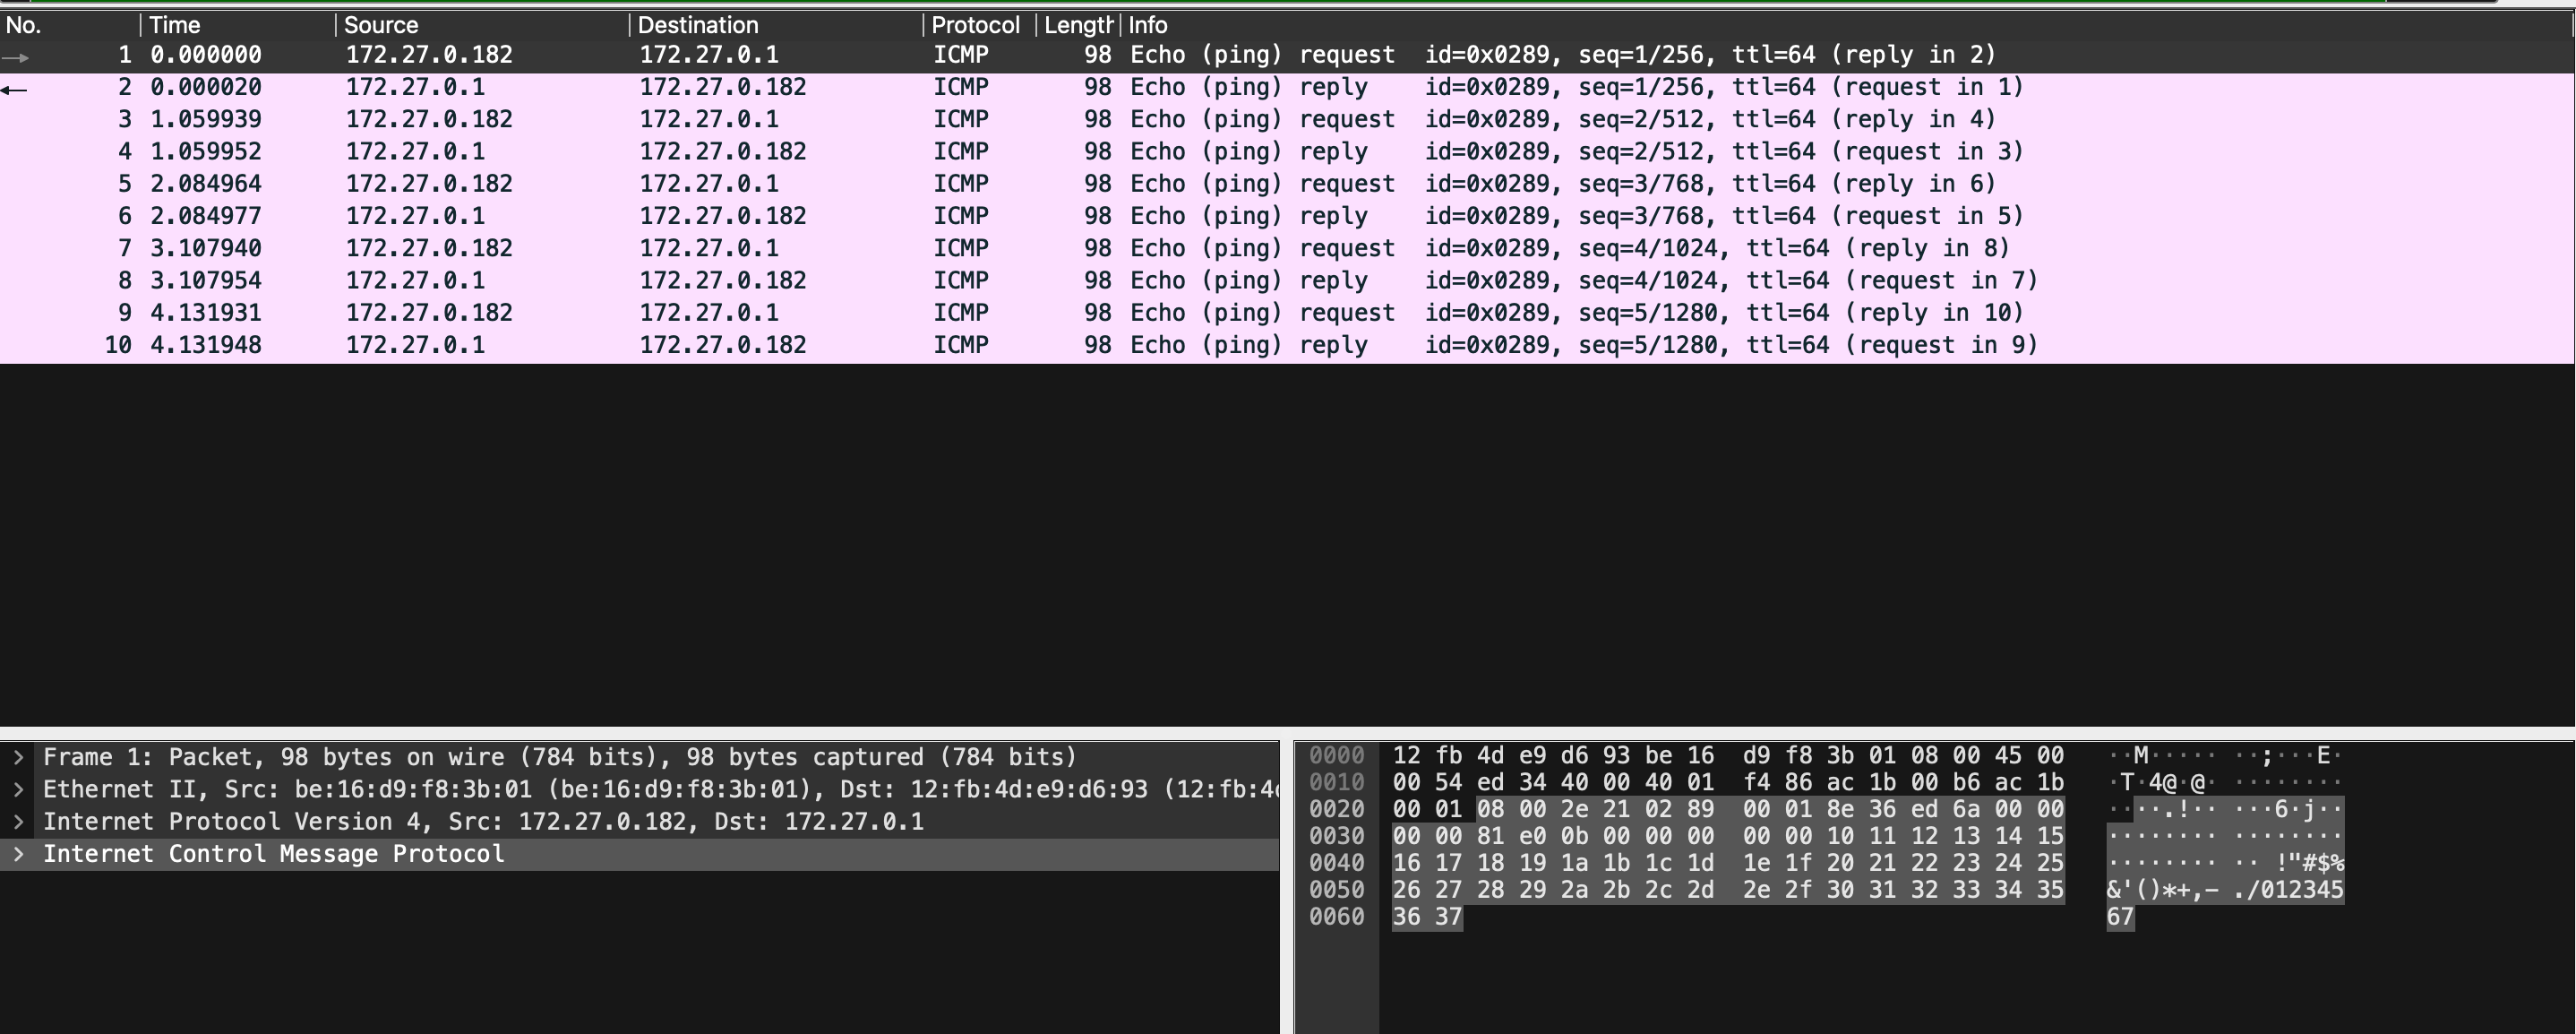
\includegraphics[width=0.98\columnwidth]{fig/wireshark_ipv4.png}
    \caption{IPv4のpingをWiresharkで読み取った結果}
    \label{fig:ws_v4}
  \end{figure}

  \begin{figure}[h]
    \centering
    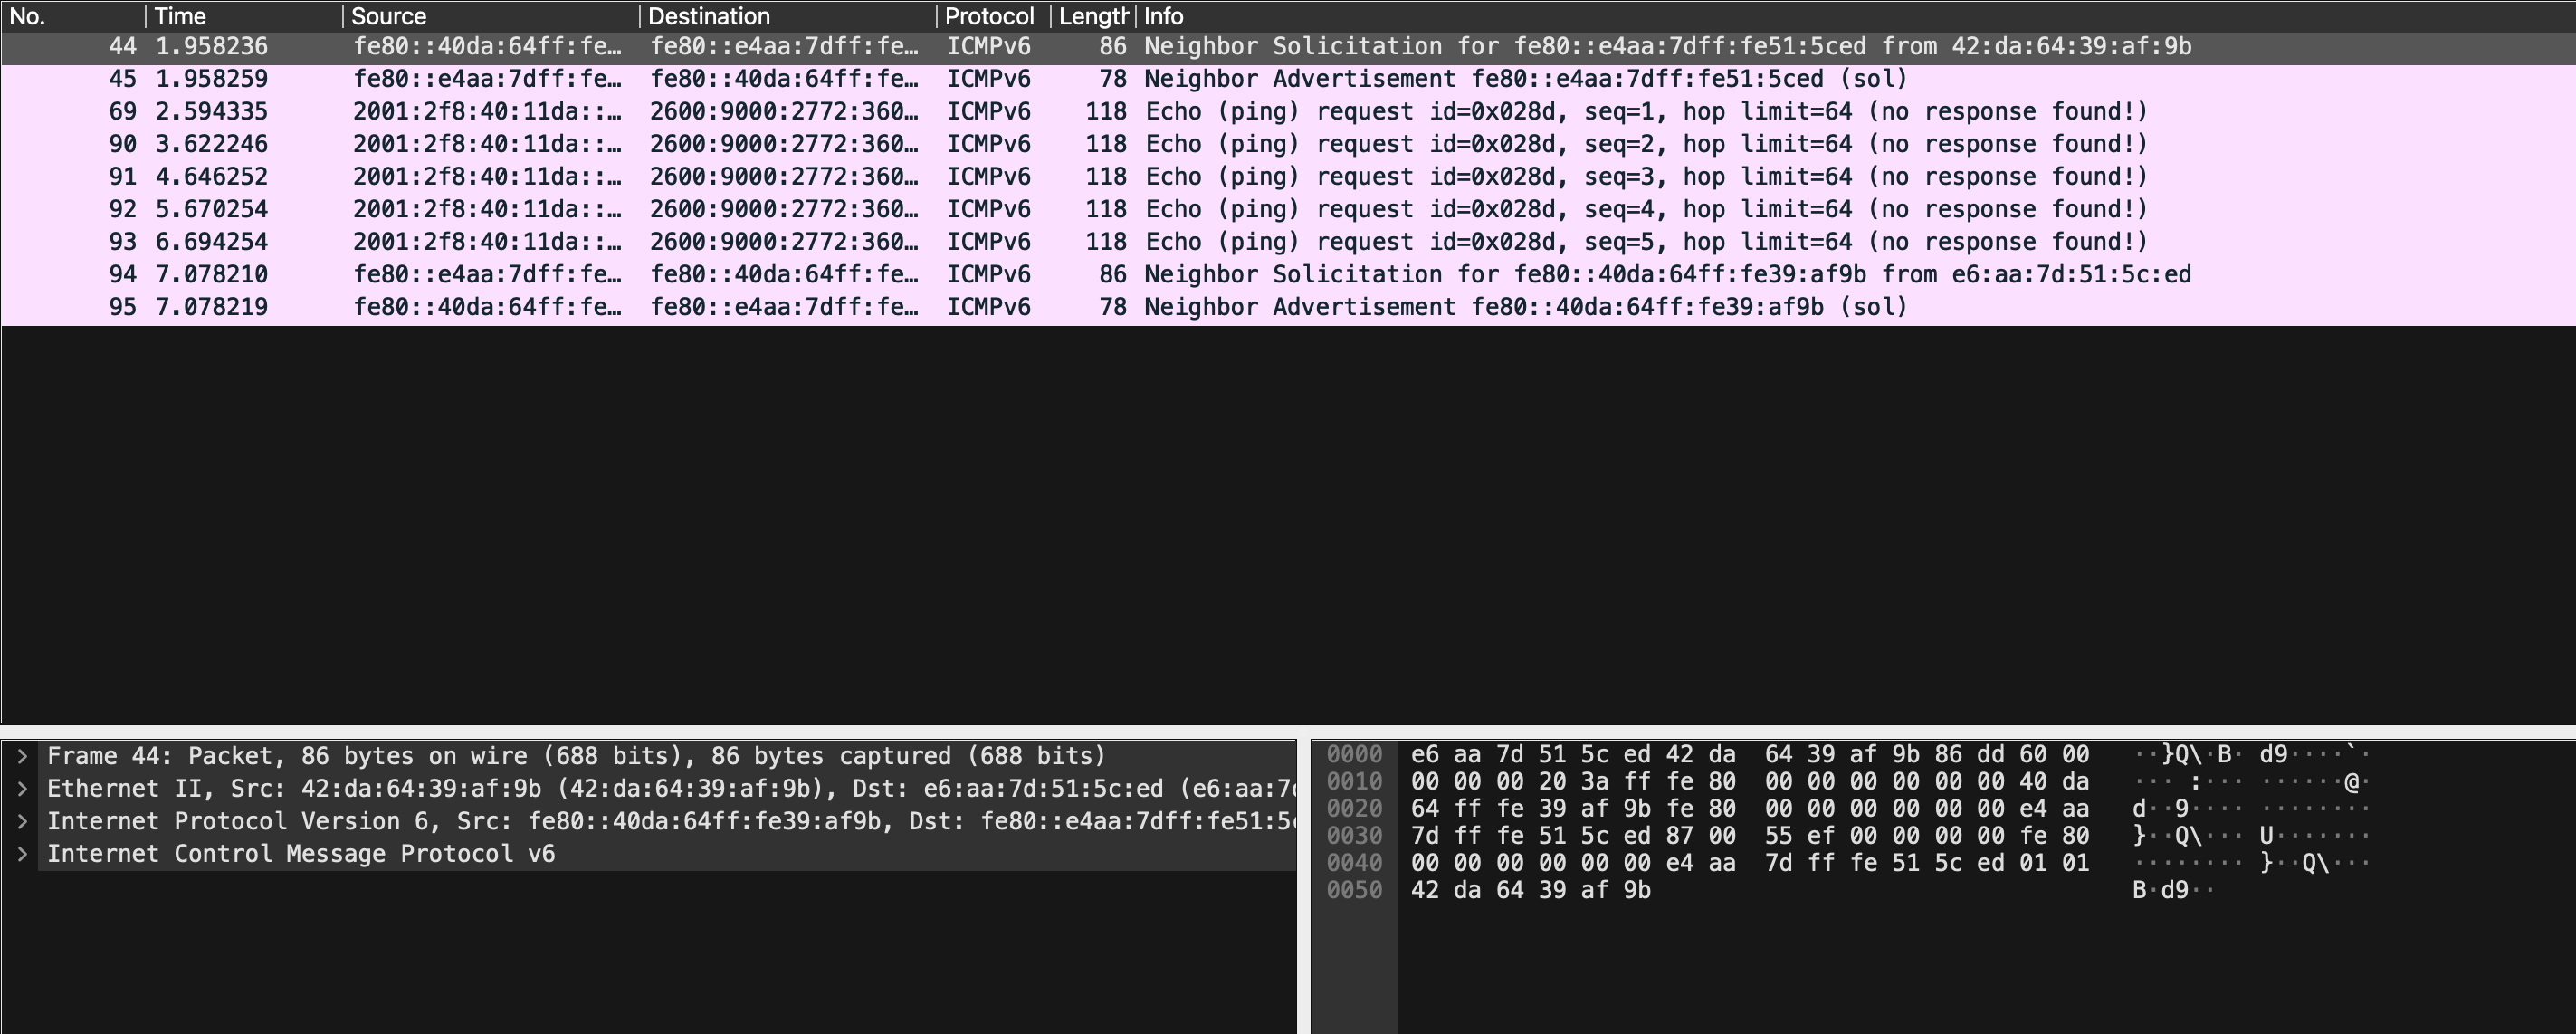
\includegraphics[width=0.98\columnwidth]{fig/wireshark_ipv6.png}
    \caption{IPv6のpingをWiresharkで読み取った結果}
    \label{fig:ws_v6}
  \end{figure}

  IPv4では，送信元172.27.0.182から172.27.0.1に向けてICMP echo requestが5回送信され，それぞれに対するecho replyが確認できた．pingの結果も5パケット送信，5パケット受信であり，パケット損失はなかった．平均往復時間は0.029ミリ秒であった．図\ref{fig:ws_v4}でも，requestとreplyが交互に並んでいることが確認できる．

  IPv6ではwww.docomo.ne.jpの名前解決はでき，2600:9000:2772:3600:7:a2b3:f240:93a1宛てのecho requestが5回送信されたが，echo replyは確認できなかった．pingの結果は5パケット送信，受信0であり，図\ref{fig:ws_v6}にもrequestのみが記録されていた．学外とのICMP通信がネットワーク上で制限されている可能性があるため，この結果だけから通信相手の停止とは判断できない．

\end{maintask}

  \begin{maintask}{1-B}
  \subsection*{課題内容}
  IPv4ではARP，IPv6では近隣探索で相手のMACアドレスを調べ，そのパケットのやり取りを確認した.

  \subsection*{実験方法}
  \begin{enumerate}
    \item 実行前の近隣キャッシュを記録
      \begin{minted}{zsh}
        ip ne
      \end{minted}

    \item 1つ目のターミナルでキャプチャを開始
      \begin{minted}{zsh}
        tcpdump -i eth1 -s 0 -w B.pcap 'not port 4200'
      \end{minted}

    \item キャプチャ中に，別のターミナルでarping，ndisc6を実行
      \begin{minted}{zsh}
        (IPv4) arping -c 3 172.28.0.200
        (IPv6) ndisc6 2001:2f8:40:11da::200 eth1
      \end{minted}

    \item 実行後に近隣キャッシュを再度記録
      \begin{minted}{zsh}
        ip ne
      \end{minted}

    \item キャプチャ側でCtrl-Cを押し，pcapをダウンロードしてWiresharkで開く
  \end{enumerate}

  \subsection*{結果}
  tcpdumpの実行結果，実行前後の近隣キャッシュ，arpingとndisc6の実行結果をそれぞれ
  出力\ref{out:tcpdump_b}，
  出力\ref{out:ne_before}，
  出力\ref{out:arping}，
  出力\ref{out:ndisc6}，
  出力\ref{out:ne_after}
  に示した．

  \begin{termout}[H]
    \caption{tcpdump の実行結果}\label{out:tcpdump_b}
    \begin{minted}{zsh}
    guest@host82:~$ tcpdump -i eth1 -s 0 -w B.pcap 'not port 4200'
    tcpdump: listening on eth1, link-type EN10MB (Ethernet), capture size 262144 bytes
    ^C498 packets captured
    500 packets received by filter
    0 packets dropped by kernel
    \end{minted}
  \end{termout}

  \begin{termout}[H]
    \caption{実行前の近隣キャッシュ}\label{out:ne_before}
    \begin{minted}{zsh}
    guest@host82:~$ ip ne
    172.28.0.203 dev eth1 lladdr e6:aa:7d:51:5c:ed STALE
    172.28.0.200 dev eth1 lladdr fe:89:01:c2:83:3a STALE
    172.28.0.1 dev eth1 lladdr a2:1e:33:b9:98:ef REACHABLE
    fe80::e4aa:7dff:fe51:5ced dev eth1 lladdr e6:aa:7d:51:5c:ed REACHABLE
    fe80::a01e:33ff:feb9:98ef dev eth1 lladdr a2:1e:33:b9:98:ef router REACHABLE
    2001:2f8:40:11da::1 dev eth1 lladdr a2:1e:33:b9:98:ef router REACHABLE
    \end{minted}
  \end{termout}

  \begin{termout}[H]
    \caption{arping(IPv4) の実行結果}\label{out:arping}
    \begin{minted}{zsh}
    guest@host82:~$ arping -c 3 172.28.0.200
    ARPING 172.28.0.200 送信元 172.28.0.182 eth1
    ユニキャスト 応答 送信元 172.28.0.200 [FE:89:01:C2:83:3A]  0.742ミリ秒
    ユニキャスト 応答 送信元 172.28.0.200 [FE:89:01:C2:83:3A]  0.522ミリ秒
    ユニキャスト 応答 送信元 172.28.0.200 [FE:89:01:C2:83:3A]  0.520ミリ秒
    3 プローブを送信 (1 ブロードキャスト)
    3 応答を受信
    \end{minted}
  \end{termout}

  \begin{termout}[H]
    \caption{ndisc6(IPv6) の実行結果}\label{out:ndisc6}
    \begin{minted}{zsh}
    guest@host82:~$ ndisc6 2001:2f8:40:11da::200 eth1
    Soliciting 2001:2f8:40:11da::200 (2001:2f8:40:11da::200) on eth1...
    Target link-layer address: FE:89:01:C2:83:3A
    from 2001:2f8:40:11da::200
    \end{minted}
  \end{termout}

  \begin{termout}[H]
    \caption{実行後の近隣キャッシュ}\label{out:ne_after}
    \begin{minted}{zsh}
    guest@host82:~$ ip ne
    172.28.0.203 dev eth1 lladdr e6:aa:7d:51:5c:ed STALE
    172.28.0.200 dev eth1 lladdr fe:89:01:c2:83:3a STALE
    172.28.0.1 dev eth1 lladdr a2:1e:33:b9:98:ef REACHABLE
    fe80::fc89:1ff:fec2:833a dev eth1 lladdr fe:89:01:c2:83:3a REACHABLE
    fe80::e4aa:7dff:fe51:5ced dev eth1 lladdr e6:aa:7d:51:5c:ed STALE
    fe80::a01e:33ff:feb9:98ef dev eth1 lladdr a2:1e:33:b9:98:ef router REACHABLE
    2001:2f8:40:11da::1 dev eth1 lladdr a2:1e:33:b9:98:ef router DELAY
    \end{minted}
  \end{termout}

  \begin{figure}[htbp]
    \centering
    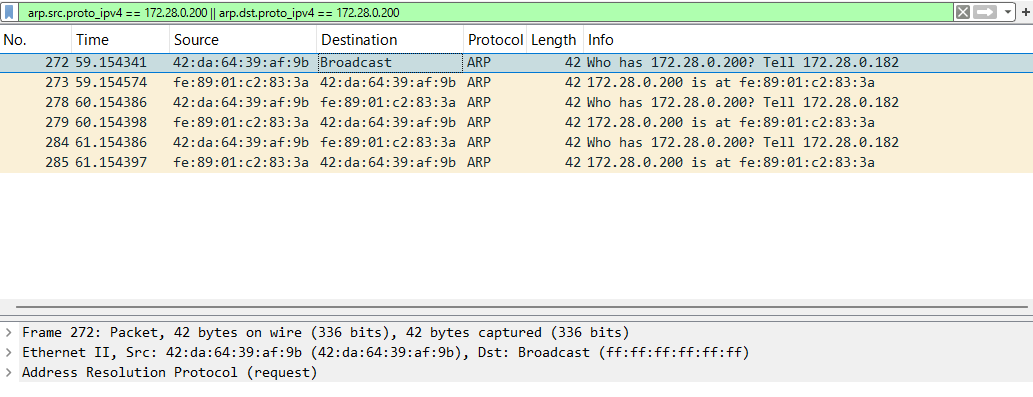
\includegraphics[width=0.98\columnwidth]{fig/wireshark_arp.png}
    \caption{ARPのやり取りをWiresharkで読み取った結果}
    \label{fig:ws_arp}
  \end{figure}

  \begin{figure}[htbp]
    \centering
    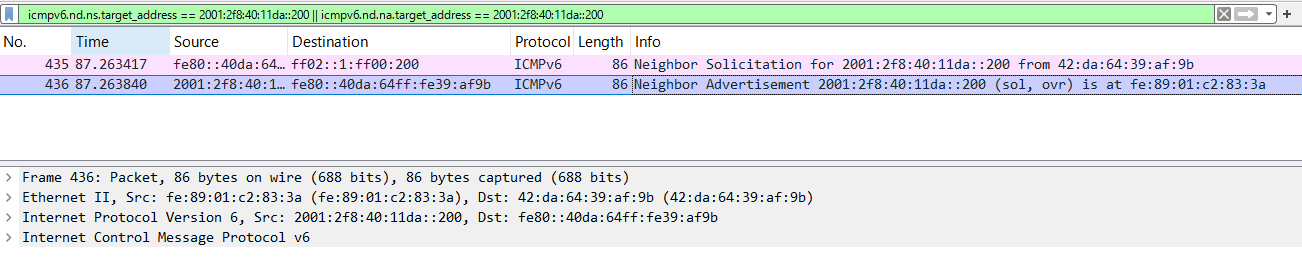
\includegraphics[width=0.98\columnwidth]{fig/wireshark_nd.png}
    \caption{NDのやり取りをWiresharkで読み取った結果}
    \label{fig:ws_nd}
  \end{figure}

  IPv4では，arpingにより172.28.0.200のMACアドレスが\texttt{FE:89:01:C2:83:3A}であると分かった．出力\ref{out:arping}には「3プローブを送信(1ブロードキャスト)」とあり，最初の1回がブロードキャストのARP Requestで，残りの2回はMACアドレスが分かった後のユニキャストであると読み取れる．図\ref{fig:ws_arp}では，No.272のARP Requestの宛先がBroadcast(ff:ff:ff:ff:ff:ff)で，``Who has 172.28.0.200? Tell 172.28.0.182''という内容になっており，No.273のARP Replyでは172.28.0.200が\texttt{fe:89:01:c2:83:3a}にいると返答している．続くNo.278とNo.284のRequestは宛先が\texttt{fe:89:01:c2:83:3a}のユニキャストで，それぞれNo.279，No.285でReplyが返っている．これは出力\ref{out:arping}の「1ブロードキャスト」の内訳と一致する．

  IPv6では，ndisc6により2001:2f8:40:11da::200のMACアドレスが，IPv4と同じ\texttt{FE:89:01:C2:83:3A}であると分かった．これはIPv4とIPv6の双方で，同一のホスト(sshd)のMACアドレスが得られたことを示す．図\ref{fig:ws_nd}では，No.435のNeighbor Solicitation(Type 135)が，宛先\texttt{ff02::1:ff00:200}（2001:2f8:40:11da::200に対するsolicited-nodeマルチキャストアドレス）に送られている．その直後のNo.436のNeighbor Advertisement(Type 136)は，2001:2f8:40:11da::200から要求元へユニキャストで返され，Target link-layer addressとして\texttt{fe:89:01:c2:83:3a}が通知されている．ARPがブロードキャストを使うのに対し，NDでは対象のアドレスに対応するマルチキャストグループ宛てにSolicitationを送る点が異なる．

  近隣キャッシュは，出力\ref{out:ne_before}と出力\ref{out:ne_after}を比べると，\texttt{fe80::fc89:1ff:fec2:833a}のエントリが新たに追加され，そのMACアドレスは上記と同じ\texttt{fe:89:01:c2:83:3a}であった．このアドレスは，MACアドレスからEUI-64形式で作られたリンクローカルアドレスである．一方，172.28.0.200のエントリは実行前から存在し(STALE)，実行後も変化していなかった．それにもかかわらず，arpingはNo.272でブロードキャストのRequestを送信している．
\end{maintask}

  \begin{maintask}{1-C}
  \subsection*{課題内容}
  LAN内のTCP echoサーバに接続し，送信した文字列がそのまま返ってくることを，IPv4・IPv6の双方で確認した．

  \subsection*{実験方法}
  \begin{enumerate}
    \item 1つ目のターミナルでキャプチャを開始
      \begin{minted}{zsh}
        tcpdump -i eth1 -s 0 -w C.pcap 'not port 4200'
      \end{minted}

    \item キャプチャ中に，別のターミナルでtelnetを実行し，適当な文字列を入力して返信を確認したのち，Ctrl+]，quitで終了する．IPv4とIPv6の双方で行う．
      \begin{minted}{zsh}
        (IPv4) telnet 172.28.0.200 echo
        (IPv6) telnet 2001:2f8:40:11da::200 echo
      \end{minted}

    \item キャプチャ側でCtrl-Cを押し，pcapをダウンロードしてWiresharkで開く
  \end{enumerate}

  \subsection*{結果}
  tcpdumpの実行結果と，IPv4・IPv6のtelnetの実行結果をそれぞれ
  出力\ref{out:tcpdump_c}，
  出力\ref{out:telnet_v4}，
  出力\ref{out:telnet_v6}
  に示した．

  \begin{termout}[H]
    \caption{tcpdump の実行結果}\label{out:tcpdump_c}
    \begin{minted}{zsh}
    guest@host82:~$ tcpdump -i eth1 -s 0 -w C.pcap 'not port 4200'
    tcpdump: listening on eth1, link-type EN10MB (Ethernet), capture size 262144 bytes
    ^C500 packets captured
    502 packets received by filter
    0 packets dropped by kernel
    \end{minted}
  \end{termout}

  \begin{termout}[H]
    \caption{telnet(IPv4) の実行結果}\label{out:telnet_v4}
    \begin{minted}{zsh}
    guest@host82:~$ telnet 172.28.0.200 echo
    Trying 172.28.0.200...
    Connected to 172.28.0.200.
    Escape character is '^]'.
    hello
    hello
    world
    world
    ^]
    telnet> quit
    Connection closed.
    \end{minted}
  \end{termout}

  \begin{termout}[H]
    \caption{telnet(IPv6) の実行結果}\label{out:telnet_v6}
    \begin{minted}{zsh}
    guest@host82:~$ telnet 2001:2f8:40:11da::200 echo
    Trying 2001:2f8:40:11da::200...
    Connected to 2001:2f8:40:11da::200.
    Escape character is '^]'.
    hoge
    hoge
    huga
    huga
    ^]
    telnet> quit
    Connection closed.
    \end{minted}
  \end{termout}

  \begin{figure}[htbp]
    \centering
    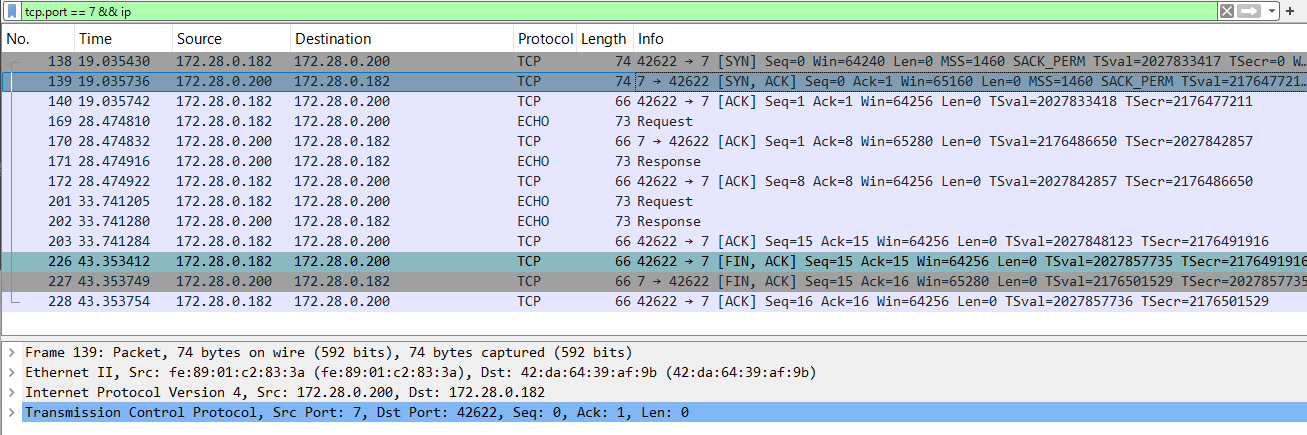
\includegraphics[width=0.98\columnwidth]{fig/wireshark_c_v4.png}
    \caption{IPv4のTCP echo通信をWiresharkで読み取った結果}
    \label{fig:ws_c_v4}
  \end{figure}

  \begin{figure}[htbp]
    \centering
    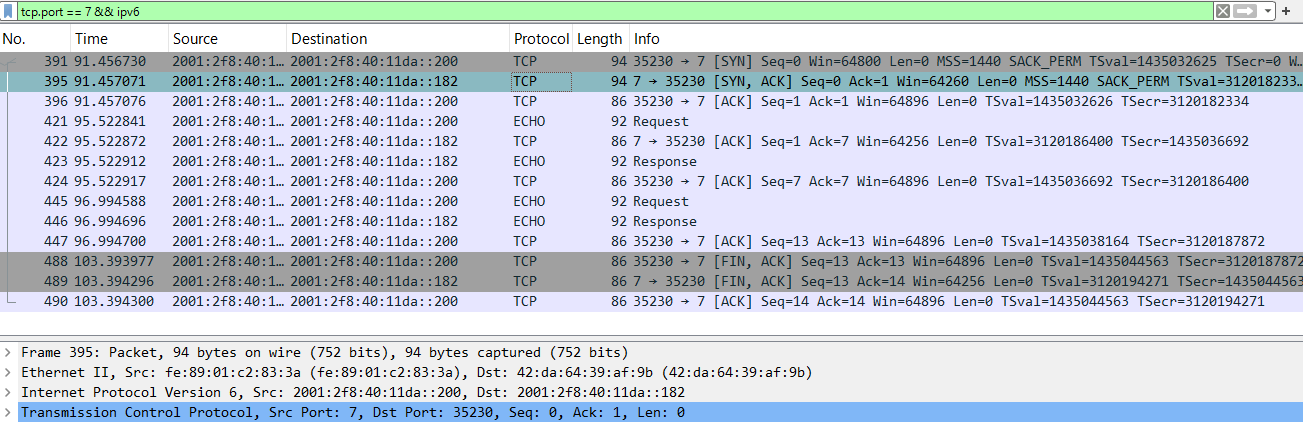
\includegraphics[width=0.98\columnwidth]{fig/wireshark_c_v6.png}
    \caption{IPv6のTCP echo通信をWiresharkで読み取った結果}
    \label{fig:ws_c_v6}
  \end{figure}

  \begin{figure}[htbp]
    \centering
    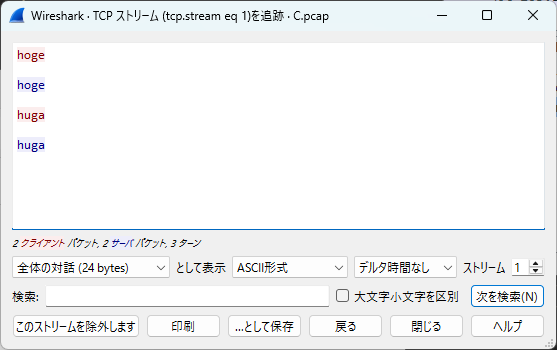
\includegraphics[width=0.7\columnwidth]{fig/wireshark_c_stream.png}
    \caption{TCPストリームの追跡結果(IPv6)}
    \label{fig:ws_c_stream}
  \end{figure}

  IPv4では，出力\ref{out:telnet_v4}のとおり，入力したhelloとworldがそれぞれそのままサーバから返ってきた．図\ref{fig:ws_c_v4}では，まずNo.138のSYN，No.139のSYN/ACK，No.140のACKにより，TCPの3ウェイハンドシェイクで接続が確立している．続いて，No.169でhelloを含むECHOのRequest（データ長7バイト）がクライアント(172.28.0.182)からサーバ(172.28.0.200)へ送られ，サーバはNo.170でACKを返したのち，No.171で同じ7バイトのResponseを返している．これをクライアントがNo.172でACKしている．worldについても同様に，No.201のRequest，No.202のResponse，No.203のACKの順にやり取りされている．データ長が7バイトであるのは，helloの5バイトに，Enterで付加される改行コード(CR LF)の2バイトが加わっているためと考えられる．最後に，クライアントがquitで接続を終了した際，No.226のFIN/ACK，No.227のFIN/ACK，No.228のACKにより接続が閉じられている．

  IPv6でも，出力\ref{out:telnet_v6}のとおり，入力したhogeとhugaがそのまま返ってきた．図\ref{fig:ws_c_v6}では，クライアント(2001:2f8:40:11da::182)とサーバ(2001:2f8:40:11da::200)の間で，IPv4と同じ手順で通信が行われている．No.391のSYN，No.395のSYN/ACK，No.396のACKで接続が確立し，No.421のRequestに対してNo.422のACK，No.423のResponse（データはいずれも6バイト），No.424のACKが続く．hugaについても，No.445のRequest，No.446のResponse，No.447のACKの順にやり取りされている．接続の終了は，No.488のFIN/ACK，No.489のFIN/ACK，No.490のACKである．図\ref{fig:ws_c_stream}のTCPストリームの追跡(IPv6)では，hogeとhugaが送信側・受信側の双方で一致して表示され，全体の対話は24バイトであった．これは，6バイトのデータが4回（送信2回，受信2回）やり取りされた合計と一致する．

  IPv4とIPv6を比べると，TCPの手順（3ウェイハンドシェイク，データの送受信，FINによる終了）は同じである．一方で，SYNパケットの長さはIPv4の74バイトに対してIPv6では94バイトと20バイト大きい．これはIPヘッダが20バイトから40バイトになったためである．また，SYNに含まれるMSSの値も，IPv4の1460に対してIPv6では1440と20バイト小さく，同じ理由で説明できる．なお，echoサービスのポート番号は7であり，いずれの通信もサーバ側のポートは7である．
\end{maintask}

  \begin{maintask}{D}
  \subsection*{課題内容}
  LAN内のiperf3サーバに対し，低速のUDP通信を順方向・逆方向(-R)の双方で行い，スループットとパケットの流れを確認した．

  \subsection*{実験方法}
  \begin{enumerate}
    \item 1つ目のターミナルでキャプチャを開始
      \begin{minted}{zsh}
        tcpdump -i eth1 -s 0 -w day2_D.pcap 'not port 4200'
      \end{minted}

    \item キャプチャ中に，別のターミナルでiperf3を順方向，逆方向の順に実行
      \begin{minted}{zsh}
        (順方向) iperf3 -t 5 -u -b 10k -c 2001:2f8:40:11da::200
        (逆方向) iperf3 -t 5 -R -u -b 10k -c 2001:2f8:40:11da::200
      \end{minted}

    \item キャプチャ側でCtrl-Cを押し，pcapをダウンロードしてWiresharkで開き，フィルタ\texttt{udp.port == 5201}を適用
  \end{enumerate}

  \subsection*{結果}
  tcpdumpの実行結果と，順方向・逆方向のiperf3の実行結果をそれぞれ
  出力\ref{out:tcpdump_d}，
  出力\ref{out:iperf_fwd}，
  出力\ref{out:iperf_rev}
  に示した．

  \begin{termout}[H]
    \caption{tcpdump の実行結果}\label{out:tcpdump_d}
    \begin{minted}{zsh}
    guest@host82:~$ tcpdump -i eth1 -s 0 -w day2_D.pcap 'not port 4200'                                      
    tcpdump: listening on eth1, link-type EN10MB (Ethernet), capture size 262144 bytes                       
    ^C520 packets captured                                                                                   
    522 packets received by filter                                                                           
    0 packets dropped by kernel  
    \end{minted}
  \end{termout}

  \begin{termout}[H]
    \caption{iperf3(順方向) の実行結果}\label{out:iperf_fwd}
    \begin{minted}{zsh}
    guest@host82:~$ iperf3 -t 5 -u -b 10k -c 2001:2f8:40:11da::200                                           
    Connecting to host 2001:2f8:40:11da::200, port 5201                                                      
    [  5] local 2001:2f8:40:11da::182 port 39751 connected to 2001:2f8:40:11da::200 port 5201                
    [ ID] Interval           Transfer     Bitrate         Total Datagrams                                    
    [  5]   0.00-1.00   sec  1.39 KBytes  11.4 Kbits/sec  1                                                  
    [  5]   1.00-2.00   sec  1.39 KBytes  11.4 Kbits/sec  1                                                  
    [  5]   2.00-3.00   sec  1.39 KBytes  11.4 Kbits/sec  1                                                  
    [  5]   3.00-4.00   sec  1.39 KBytes  11.4 Kbits/sec  1                                                  
    [  5]   4.00-5.00   sec  1.39 KBytes  11.4 Kbits/sec  1                                                  
    - - - - - - - - - - - - - - - - - - - - - - - - -                                                        
    [ ID] Interval           Transfer     Bitrate         Jitter    Lost/Total Datagrams                     
    [  5]   0.00-5.00   sec  6.97 KBytes  11.4 Kbits/sec  0.000 ms  0/5 (0%)  sender                         
    [  5]   0.00-5.04   sec  6.97 KBytes  11.3 Kbits/sec  0.003 ms  0/5 (0%)  receiver                       
                                                                                                            
    iperf Done.       
    \end{minted}
  \end{termout}

  \begin{termout}[H]
    \caption{iperf3(逆方向) の実行結果}\label{out:iperf_rev}
    \begin{minted}{zsh}
    guest@host82:~$ iperf3 -t 5 -R -u -b 10k -c 2001:2f8:40:11da::200                                        
    Connecting to host 2001:2f8:40:11da::200, port 5201                                                      
    Reverse mode, remote host 2001:2f8:40:11da::200 is sending                                               
    [  5] local 2001:2f8:40:11da::182 port 37219 connected to 2001:2f8:40:11da::200 port 5201                
    [ ID] Interval           Transfer     Bitrate         Jitter    Lost/Total Datagrams                     
    [  5]   0.00-1.00   sec  1.39 KBytes  11.4 Kbits/sec  2.541 ms  0/1 (0%)                                 
    [  5]   1.00-2.00   sec  1.39 KBytes  11.4 Kbits/sec  4.921 ms  0/1 (0%)                                 
    [  5]   2.00-3.00   sec  1.39 KBytes  11.4 Kbits/sec  4.613 ms  0/1 (0%)                                 
    [  5]   3.00-4.00   sec  1.39 KBytes  11.4 Kbits/sec  4.325 ms  0/1 (0%)                                 
    [  5]   4.00-5.00   sec  1.39 KBytes  11.4 Kbits/sec  4.055 ms  0/1 (0%)                                 
    - - - - - - - - - - - - - - - - - - - - - - - - -                                                        
    [ ID] Interval           Transfer     Bitrate         Jitter    Lost/Total Datagrams                     
    [  5]   0.00-5.04   sec  6.97 KBytes  11.3 Kbits/sec  0.000 ms  0/5 (0%)  sender                         
    [  5]   0.00-5.00   sec  6.97 KBytes  11.4 Kbits/sec  4.055 ms  0/5 (0%)  receiver                       
                                                                                                            
    iperf Done.       
    \end{minted}
  \end{termout}

  \begin{figure}[h]
    \centering
    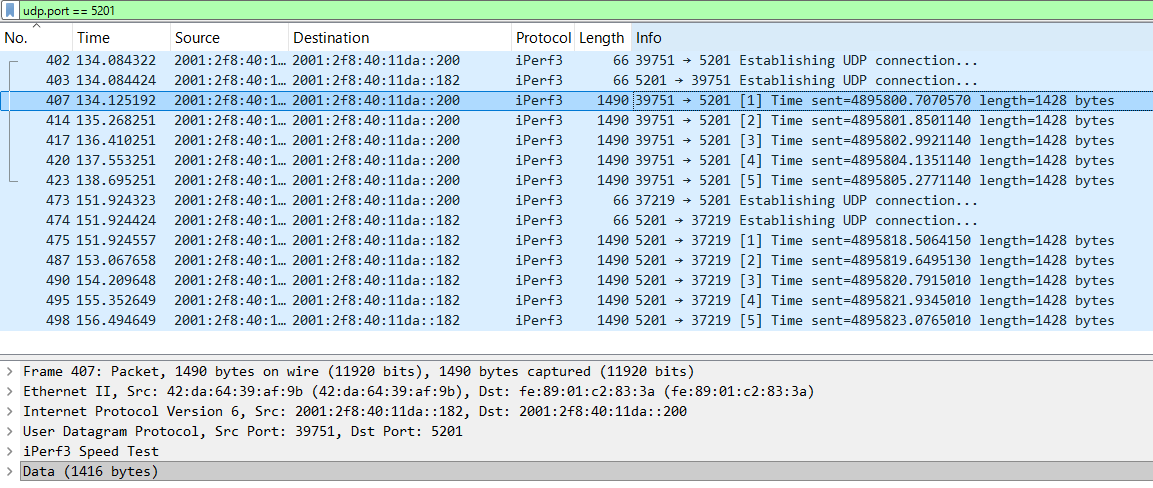
\includegraphics[width=0.98\columnwidth]{fig/wireshark_d_fwd.png}
    \caption{順方向のUDP通信をWiresharkで読み取った結果}
    \label{fig:ws_d_fwd}
  \end{figure}

  \begin{figure}[h]
    \centering
    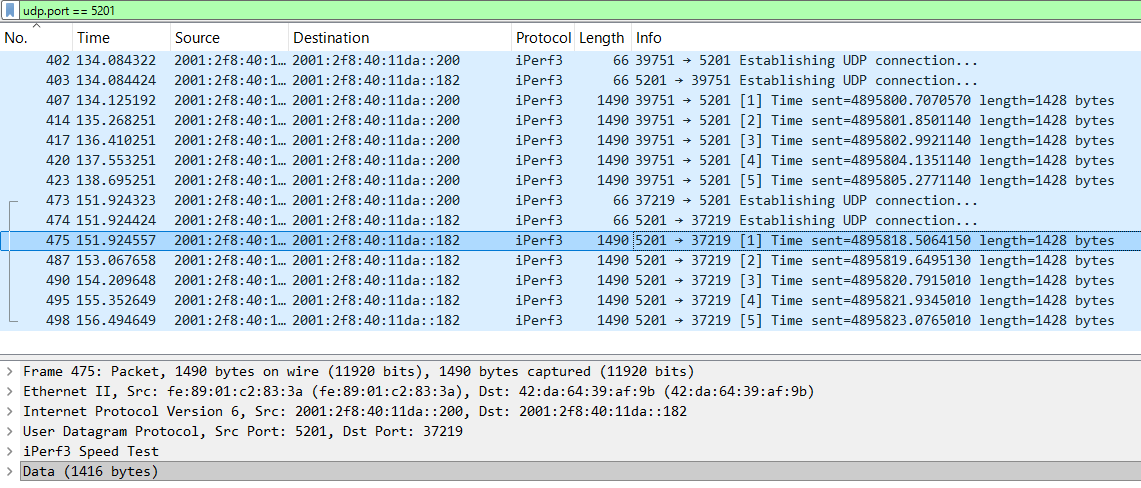
\includegraphics[width=0.98\columnwidth]{fig/wireshark_d_rev.png}
    \caption{逆方向のUDP通信をWiresharkで読み取った結果}
    \label{fig:ws_d_rev}
  \end{figure}

  順方向では，出力\ref{out:iperf_fwd}のとおり，指定した10 kbit/sに対し実測のBitrateは【要記入】であり，【要記入】個のデータグラムを送信して損失は【要記入】であった．図\ref{fig:ws_d_fwd}では，No.【要記入】でクライアント(2001:2f8:40:11da::182)からサーバ(2001:2f8:40:11da::200)のUDP 5201番ポートへ短いデータグラム(【要記入】バイト)が送られ，No.【要記入】でサーバから応答が返っており，これが接続手続きに相当する．その後，No.【要記入】〜【要記入】でデータを含むUDPパケット(ペイロード長【要記入】バイト)が約【要記入】秒間隔で送られている．ペイロード長を$L$バイトとすると，10 kbit/sを保つための送信間隔は$8L/10000$秒であり，$L=$【要記入】のとき【要記入】秒となって観測値と【一致する／しない】．

  逆方向(-R)では，データを送る側がサーバになる．図\ref{fig:ws_d_rev}では，接続手続きののち，サーバ(::200)からクライアント(::182)へデータを含むUDPパケットが送られており，パケットの向きが順方向と入れ替わっている．出力\ref{out:iperf_rev}のBitrateは【要記入】，損失は【要記入】であった．

  なお，フィルタ\texttt{udp.port == 5201}には，iperf3の制御に使われるTCPの接続は含まれない．【要記入：TCP 5201の制御接続を見て気づいたことがあれば】
\end{maintask}

  \begin{maintask}{E}
  \subsection*{課題内容}
  学外のWebサイトにwgetでHTTP/HTTPSアクセスし，通信の手順（ゲートウェイのMACアドレス解決，DNS，HTTP，HTTPS）を確認した．

  \subsection*{実験方法}
  \begin{enumerate}
    \item 経路表と近隣キャッシュを記録
      \begin{minted}{zsh}
        ip -4 route
        ip -6 route
        ip ne
      \end{minted}

    \item 以下のサイトごとに，キャプチャ開始，wget実行，キャプチャ停止を繰り返す（pcapはサイトごとに分ける）．tcpdumpとwgetは別のターミナルで実行し，wgetの終了後にCtrl-Cでキャプチャを止める．
      \begin{minted}{zsh}
        (IPv4のみ)    tcpdump -i eth1 -s 0 -w day2_E_sapporo.pcap 'not port 4200'
                      wget www.city.sapporo.jp
        (IPv4/IPv6)   tcpdump -i eth1 -s 0 -w day2_E_hokkaido.pcap 'not port 4200'
                      wget www.pref.hokkaido.lg.jp
        (IPv6のみ指定) tcpdump -i eth1 -s 0 -w day2_E_keio.pcap 'not port 4200'
                      wget www.keio.ac.jp
      \end{minted}
      % TODO: keioは「IPv6のみ指定」。実際に -6 を付けたならここも wget -6 www.keio.ac.jp に直す

    \item 各pcapをWiresharkで開き，次のフィルタを適用
      \begin{minted}{text}
        (arp || icmpv6.type == 135 || icmpv6.type == 136 || dns || tcp.port == 80 || tcp.port == 443) && !(dns.qry.type == 12)
      \end{minted}
  \end{enumerate}

  \subsection*{結果}
  実行前の経路表と近隣キャッシュを出力\ref{out:route_e}に，サイトごとのtcpdumpとwgetの実行結果を
  出力\ref{out:e_sapporo}，
  出力\ref{out:e_hokkaido}，
  出力\ref{out:e_keio}
  に示した．

  \begin{termout}[H]
    \caption{実行前の経路表と近隣キャッシュ}\label{out:route_e}
    \begin{minted}{zsh}
    guest@host82:~$ ip -4 route
    default via 172.28.0.1 dev eth1                                                                          
    172.27.0.0/24 dev eth0 proto kernel scope link src 172.27.0.182                                          
    172.28.0.0/24 dev eth1 proto kernel scope link src 172.28.0.182                                          

    guest@host82:~$ ip -6 route                                                                              
    2001:2f8:40:11da::/64 dev eth1 proto kernel metric 256 pref medium                                       
    fe80::/64 dev eth1 proto kernel metric 256 pref medium                                                   
    default via 2001:2f8:40:11da::1 dev eth1 metric 1024 pref medium                                         

    guest@host82:~$ ip ne                                                                                    
    172.28.0.203 dev eth1 lladdr e6:aa:7d:51:5c:ed STALE                                                     
    172.28.0.1 dev eth1 lladdr a2:1e:33:b9:98:ef REACHABLE                                                   
    fe80::fc89:1ff:fec2:833a dev eth1 lladdr fe:89:01:c2:83:3a STALE                                         
    2001:2f8:40:11da::200 dev eth1 lladdr fe:89:01:c2:83:3a STALE                                            
    2001:2f8:40:11da::203 dev eth1 lladdr e6:aa:7d:51:5c:ed STALE                                            
    fe80::e4aa:7dff:fe51:5ced dev eth1 lladdr e6:aa:7d:51:5c:ed REACHABLE                                    
    fe80::a01e:33ff:feb9:98ef dev eth1 lladdr a2:1e:33:b9:98:ef router REACHABLE                             
    2001:2f8:40:11da::1 dev eth1 lladdr a2:1e:33:b9:98:ef router REACHABLE        
    \end{minted}
  \end{termout}

  \begin{termout}[H]
    \caption{www.city.sapporo.jp の tcpdump と wget の実行結果}\label{out:e_sapporo}
    \begin{minted}{zsh}
    guest@host82:~$ tcpdump -i eth1 -s 0 -w day2_E_sapporo.pcap 'not port 4200'
    tcpdump: listening on eth1, link-type EN10MB (Ethernet), capture size 262144 bytes
    ^C152 packets captured
    154 packets received by filter
    0 packets dropped by kernel

    guest@host82:~$ wget www.city.sapporo.jp
    --2026-11-10 00:55:19--  http://www.city.sapporo.jp/
    www.city.sapporo.jp (www.city.sapporo.jp) をDNSに問いあわせています... 45.60.112.77
    www.city.sapporo.jp (www.city.sapporo.jp)|45.60.112.77|:80 に接続しています... 接続しました。
    HTTP による接続要求を送信しました、応答を待っています... 301 Moved Permanently
    場所: https://www.city.sapporo.jp/ [続く]
    --2026-11-10 00:55:19--  https://www.city.sapporo.jp/
    www.city.sapporo.jp (www.city.sapporo.jp)|45.60.112.77|:443 に接続しています... 接続しました。
    HTTP による接続要求を送信しました、応答を待っています... 200 OK
    長さ: 38349 (37K) [text/html]
    `index.html' に保存中

    index.html                 100%[=====================================>]  37.45K  --.-KB/s    in 0.03s   

    2026-11-10 00:55:20 (1.27 MB/s) - `index.html' へ保存完了 [38349/38349]
    \end{minted}
  \end{termout}

  \begin{termout}[H]
    \caption{www.pref.hokkaido.lg.jp の tcpdump と wget の実行結果}\label{out:e_hokkaido}
    \begin{minted}{zsh}
    guest@host82:~$ tcpdump -i eth1 -s 0 -w day2_E_hokkaido.pcap 'not port 4200'
    tcpdump: listening on eth1, link-type EN10MB (Ethernet), capture size 262144 bytes
    ^C170 packets captured
    172 packets received by filter
    0 packets dropped by kernel

    guest@host82:~$ wget www.pref.hokkaido.lg.jp
    --2026-11-10 00:57:19--  http://www.pref.hokkaido.lg.jp/
    www.pref.hokkaido.lg.jp (www.pref.hokkaido.lg.jp) をDNSに問いあわせています... 2a02:e980:10e::4d, 45.60.112.77
    www.pref.hokkaido.lg.jp (www.pref.hokkaido.lg.jp)|2a02:e980:10e::4d|:80 に接続しています... 接続しました。
    HTTP による接続要求を送信しました、応答を待っています... 302 Found
    場所: https://www.pref.hokkaido.lg.jp/ [続く]
    --2026-11-10 00:57:19--  https://www.pref.hokkaido.lg.jp/
    www.pref.hokkaido.lg.jp (www.pref.hokkaido.lg.jp)|2a02:e980:10e::4d|:443 に接続しています... 接続しました。
    HTTP による接続要求を送信しました、応答を待っています... 200 OK
    長さ: 特定できません [text/html]
    `index.html.1' に保存中

    index.html.1                   [ <=>                                  ]  93.46K  --.-KB/s    in 0.07s   

    2026-11-10 00:57:20 (1.40 MB/s) - `index.html.1' へ保存終了 [95704]
    \end{minted}
  \end{termout}

  \begin{termout}[H]
    \caption{www.keio.ac.jp の tcpdump と wget の実行結果}\label{out:e_keio}
    \begin{minted}{zsh}
    guest@host82:~$ tcpdump -i eth1 -s 0 -w day2_E_keio.pcap 'not port 4200'
    tcpdump: listening on eth1, link-type EN10MB (Ethernet), capture size 262144 bytes
    ^C296 packets captured
    298 packets received by filter
    0 packets dropped by kernel

    guest@host82:~$ wget www.keio.ac.jp
    --2026-11-10 00:59:01--  http://www.keio.ac.jp/
    www.keio.ac.jp (www.keio.ac.jp) をDNSに問いあわせています... 2600:9000:2142:5800:9:dcf4:5ec0:93a1, 2600:9000:2142:50
    00:9:dcf4:5ec0:93a1, 2600:9000:2142:3c00:9:dcf4:5ec0:93a1, ...
    www.keio.ac.jp (www.keio.ac.jp)|2600:9000:2142:5800:9:dcf4:5ec0:93a1|:80 に接続しています... 接続しました。
    HTTP による接続要求を送信しました、応答を待っています... 301 Moved Permanently
    場所: https://www.keio.ac.jp/ [続く]
    --2026-11-10 00:59:01--  https://www.keio.ac.jp/
    www.keio.ac.jp (www.keio.ac.jp)|2600:9000:2142:5800:9:dcf4:5ec0:93a1|:443 に接続しています... 接続しました。
    HTTP による接続要求を送信しました、応答を待っています... 301 Moved Permanently
    場所: /ja/ [続く]
    --2026-11-10 00:59:01--  https://www.keio.ac.jp/ja/
    [www.keio.ac.jp]:443 への接続を再利用します。
    HTTP による接続要求を送信しました、応答を待っています... 200 OK
    長さ: 372926 (364K) [text/html]
    `index.html.2' に保存中

    index.html.2               100%[=====================================>] 364.19K  --.-KB/s    in 0.05s   

    2026-11-10 00:59:01 (6.60 MB/s) - `index.html.2' へ保存完了 [372926/372926]
  \end{minted}
  \end{termout}

  \begin{figure}[h]
    \centering
    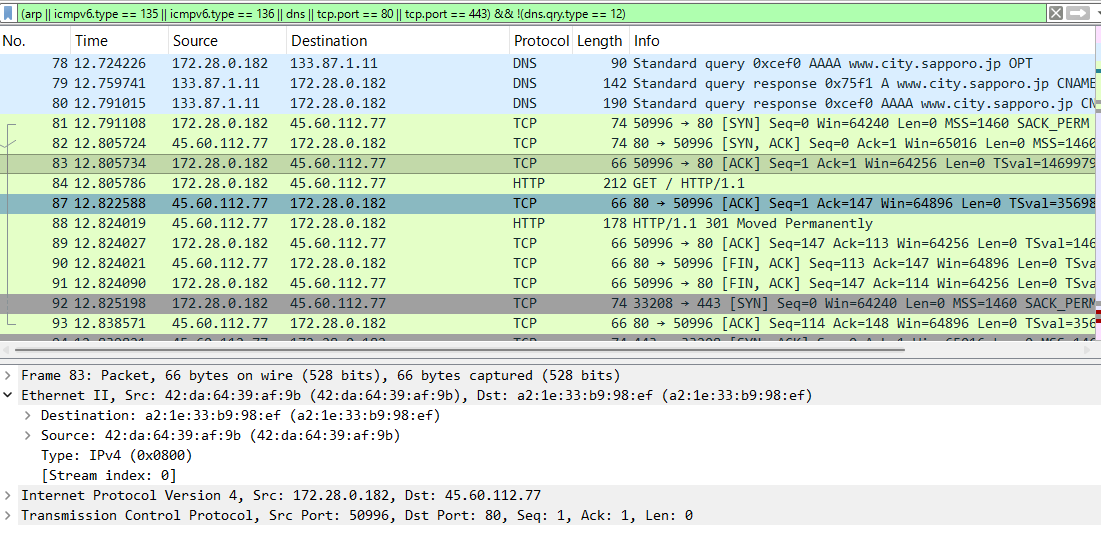
\includegraphics[width=0.98\columnwidth]{fig/wireshark_e_sapporo.png}
    \caption{www.city.sapporo.jpへのアクセスをWiresharkで読み取った結果}
    \label{fig:ws_e_sapporo}
  \end{figure}

  \begin{figure}[h]
    \centering
    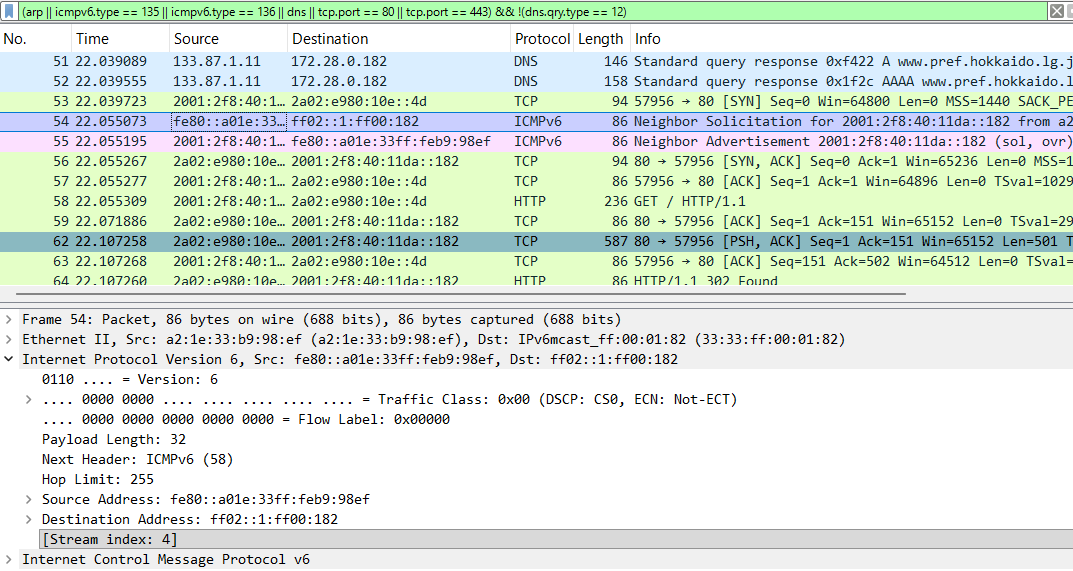
\includegraphics[width=0.98\columnwidth]{fig/wireshark_e_hokkaido.png}
    \caption{www.pref.hokkaido.lg.jpへのアクセスをWiresharkで読み取った結果}
    \label{fig:ws_e_hokkaido}
  \end{figure}

  \begin{figure}[h]
    \centering
    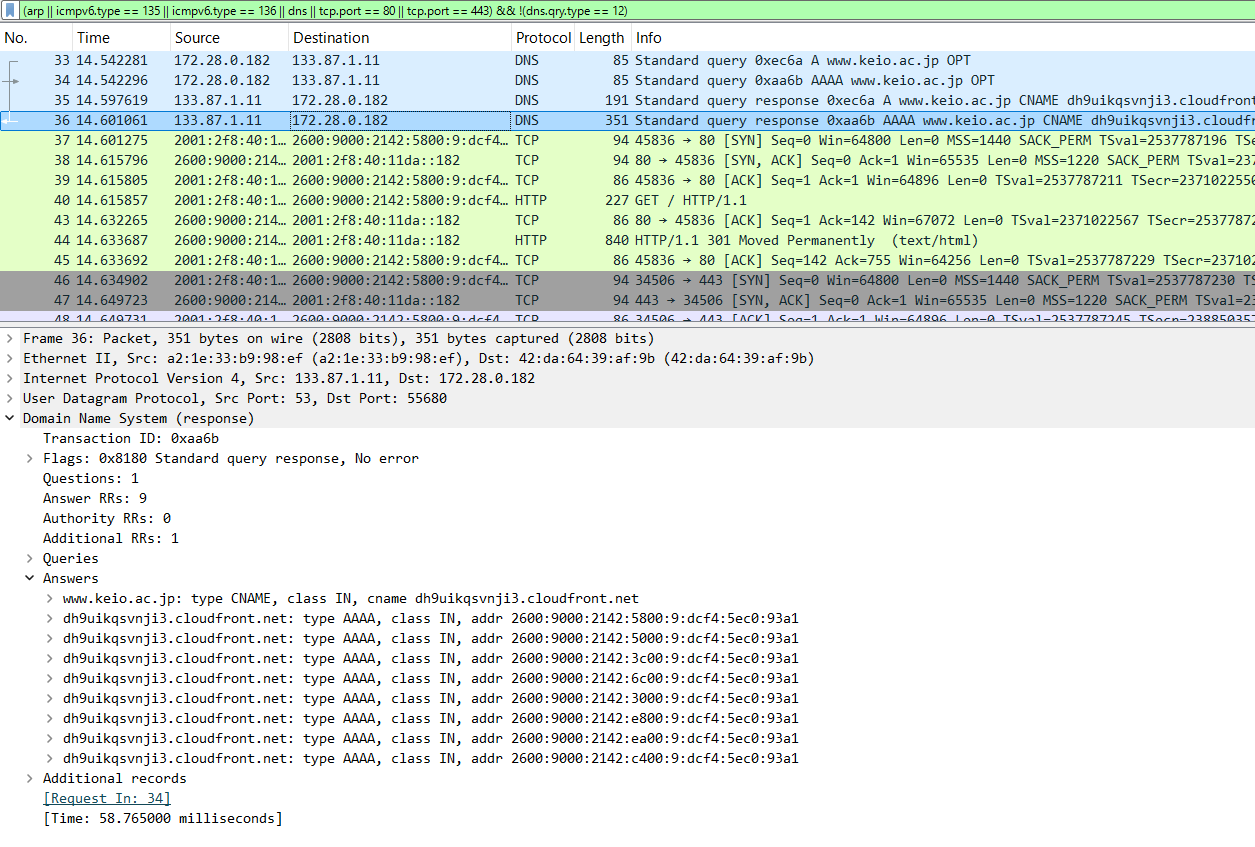
\includegraphics[width=0.98\columnwidth]{fig/wireshark_e_keio.png}
    \caption{www.keio.ac.jpへのアクセスをWiresharkで読み取った結果}
    \label{fig:ws_e_keio}
  \end{figure}

  学外への通信は，まずデフォルトゲートウェイのMACアドレスを解決することから始まる．出力\ref{out:route_e}の経路表では，デフォルトゲートウェイはIPv4が【要記入】，IPv6が【要記入】であり，近隣キャッシュには両者のMACアドレス【要記入】がすでに登録されていた．そのため，図\ref{fig:ws_e_sapporo}〜図\ref{fig:ws_e_keio}では【ARP/NDのパケットが現れなかった／現れた】．【現れなかった場合：キャッシュの内容(出力\ref{out:route_e})から，ゲートウェイのMACアドレスは既知であったと言える．】

  www.city.sapporo.jpでは，図\ref{fig:ws_e_sapporo}のNo.【要記入】で名前解決のためAレコードの問い合わせがDNSリゾルバ【要記入】に送られ，No.【要記入】の応答でアドレス【要記入】が得られた．AAAAレコードの問い合わせ(No.【要記入】)に対する応答は【アドレスなし】であり，このサイトはIPv4のみに対応していることが分かる．続いて，TCPの接続後にHTTPのGETがポート80に送られ，No.【要記入】のレスポンスは【要記入：301などのステータスコードとLocation】であった．【HTTPSへ転送されている場合：その後ポート443へ接続し，TLSハンドシェイク(Client Hello，Server Hello，Certificate等)ののちHTTPSでコンテンツが取得された．】

  www.pref.hokkaido.lg.jpは，図\ref{fig:ws_e_hokkaido}のとおりAとAAAAの双方に応答があり，IPv4/IPv6の両方に対応している．wgetが実際に使用したのは【IPv4／IPv6】で，その理由は【要記入】と考えられる．HTTPおよびHTTPSの手順は【要記入】．

  www.keio.ac.jpについては，図\ref{fig:ws_e_keio}で【要記入：問い合わせるレコード，使用したIPバージョン，HTTP/HTTPSの手順】．

  以上より，【3サイトの違い（IPバージョン，リダイレクトの有無，TLSのバージョンなど）を2〜3文でまとめる】．
\end{maintask}

  \begin{maintask}{3-1}
  \subsection*{課題内容}
  PythonのDNSリゾルバ(dnspython)で，IPv4のみ対応のホストとIPv4/IPv6両対応のホストのA・AAAAレコードを引き，その通信を分析した．

  \subsection*{実験方法}
  \begin{enumerate}
    \item ひな型を自分のホームにコピー
      \begin{minted}{zsh}
        cd; cp -r /shares/dns .; chmod -R u+w dns; cd dns
      \end{minted}

    \item ホスト名ごとに，キャプチャ開始，q\_hostnameの書き換え，実行，キャプチャ停止を行う
      \begin{minted}{zsh}
        (IPv4のみ)  tcpdump -i eth1 -s 0 -w day3_1_v4.pcap 'not port 4200'    (1つ目のターミナル)
                    sed -i "s/^q_hostname=.*/q_hostname='www.city.sapporo.jp'/" dnspython_sample.py
                    ./dnspython_sample.py
        (両対応)    tcpdump -i eth1 -s 0 -w day3_1_v46.pcap 'not port 4200'   (1つ目のターミナル)
                    sed -i "s/^q_hostname=.*/q_hostname='www.pref.hokkaido.lg.jp'/" dnspython_sample.py
                    ./dnspython_sample.py
      \end{minted}

    \item 各pcapをWiresharkで開き，次のフィルタを適用
      \begin{minted}{text}
        udp.port == 53 && !(dns.qry.type == 12)
      \end{minted}
      逆引き(PTR, Type 12)は本課題と無関係なので除外した．
  \end{enumerate}

  \subsection*{結果}
  tcpdumpの実行結果と，dnspython\_sample.pyの実行結果を
  出力\ref{out:tcpdump_31_v4}，
  出力\ref{out:tcpdump_31_v46}，
  出力\ref{out:dnspy_v4}，
  出力\ref{out:dnspy_v46}
  に示した．

  \begin{termout}[H]
    \caption{tcpdump(IPv4のみのホスト) の実行結果}\label{out:tcpdump_31_v4}
    \begin{minted}{zsh}
    guest@host82:~/dns$ tcpdump -i eth1 -s 0 -w day3_1_v4.pcap 'not port 4200'
    tcpdump: listening on eth1, link-type EN10MB (Ethernet), capture size 262144 bytes
    ^C58 packets captured
    60 packets received by filter
    0 packets dropped by kernel
    \end{minted}
  \end{termout}

  \begin{termout}[H]
    \caption{tcpdump(両対応のホスト) の実行結果}\label{out:tcpdump_31_v46}
    \begin{minted}{zsh}
    guest@host82:~/dns$ tcpdump -i eth1 -s 0 -w day3_1_v46.pcap 'not port 4200'
    tcpdump: listening on eth1, link-type EN10MB (Ethernet), capture size 262144 bytes
    ^C22 packets captured
    24 packets received by filter
    0 packets dropped by kernel
    \end{minted}
  \end{termout}

  \begin{termout}[H]
    \caption{dnspython\_sample.py(www.city.sapporo.jp) の実行結果}\label{out:dnspy_v4}
    \begin{minted}{zsh}
    guest@host82:~/dns$ ./dnspython_sample.py
    Querying hostname: www.city.sapporo.jp
    A records are:
      45.60.112.77
      Replied nameserver: 133.87.1.11 (53)
    AAAA records: No answer from the resolver.
    \end{minted}
  \end{termout}

  \begin{termout}[H]
    \caption{dnspython\_sample.py(www.pref.hokkaido.lg.jp) の実行結果}\label{out:dnspy_v46}
    \begin{minted}{zsh}
    guest@host82:~/dns$ ./dnspython_sample.py
    Querying hostname: www.pref.hokkaido.lg.jp
    A records are:
      45.60.112.77
      Replied nameserver: 133.87.1.11 (53)
    AAAA records are:
      2a02:e980:10e::4d
      Replied nameserver: 133.87.1.11 (53)
    \end{minted}
  \end{termout}

  \begin{figure}[h]
    \centering
    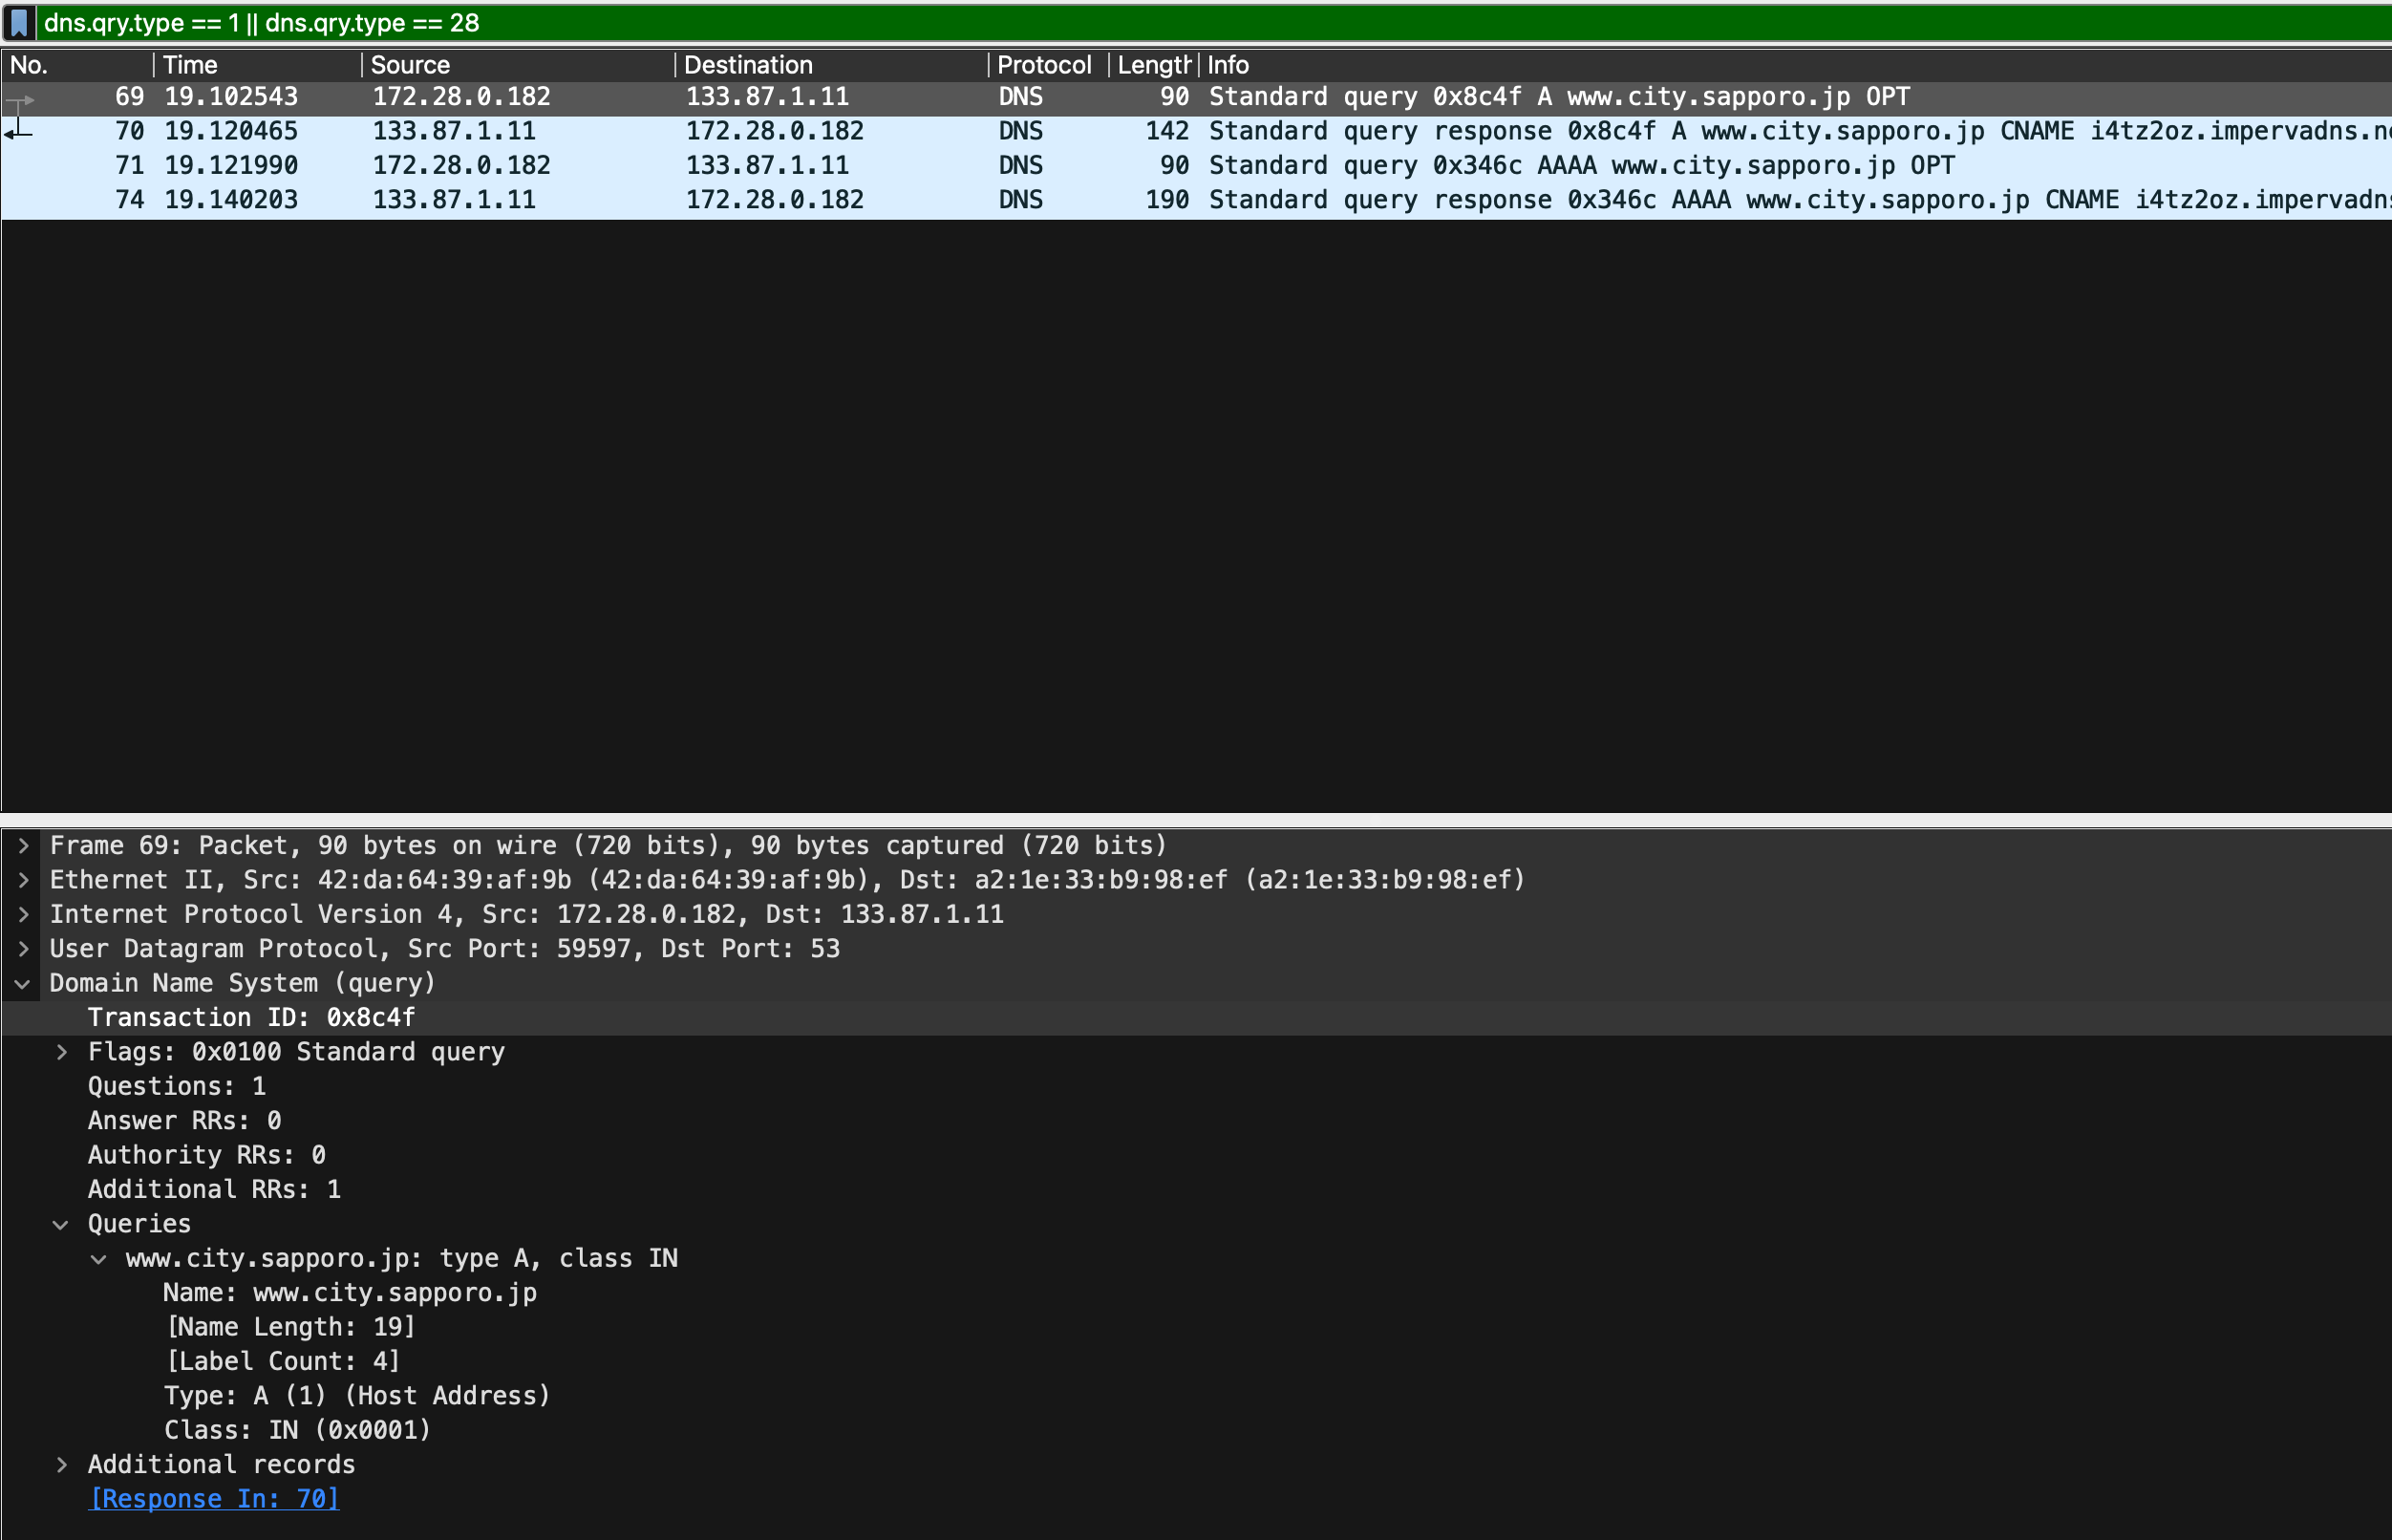
\includegraphics[width=0.98\columnwidth]{fig/wireshark_31_v4_query.png}
    \caption{IPv4のみのホストのA・AAAAの問い合わせ}
    \label{fig:ws_31_v4_query}
  \end{figure}

  \begin{figure}[h]
    \centering
    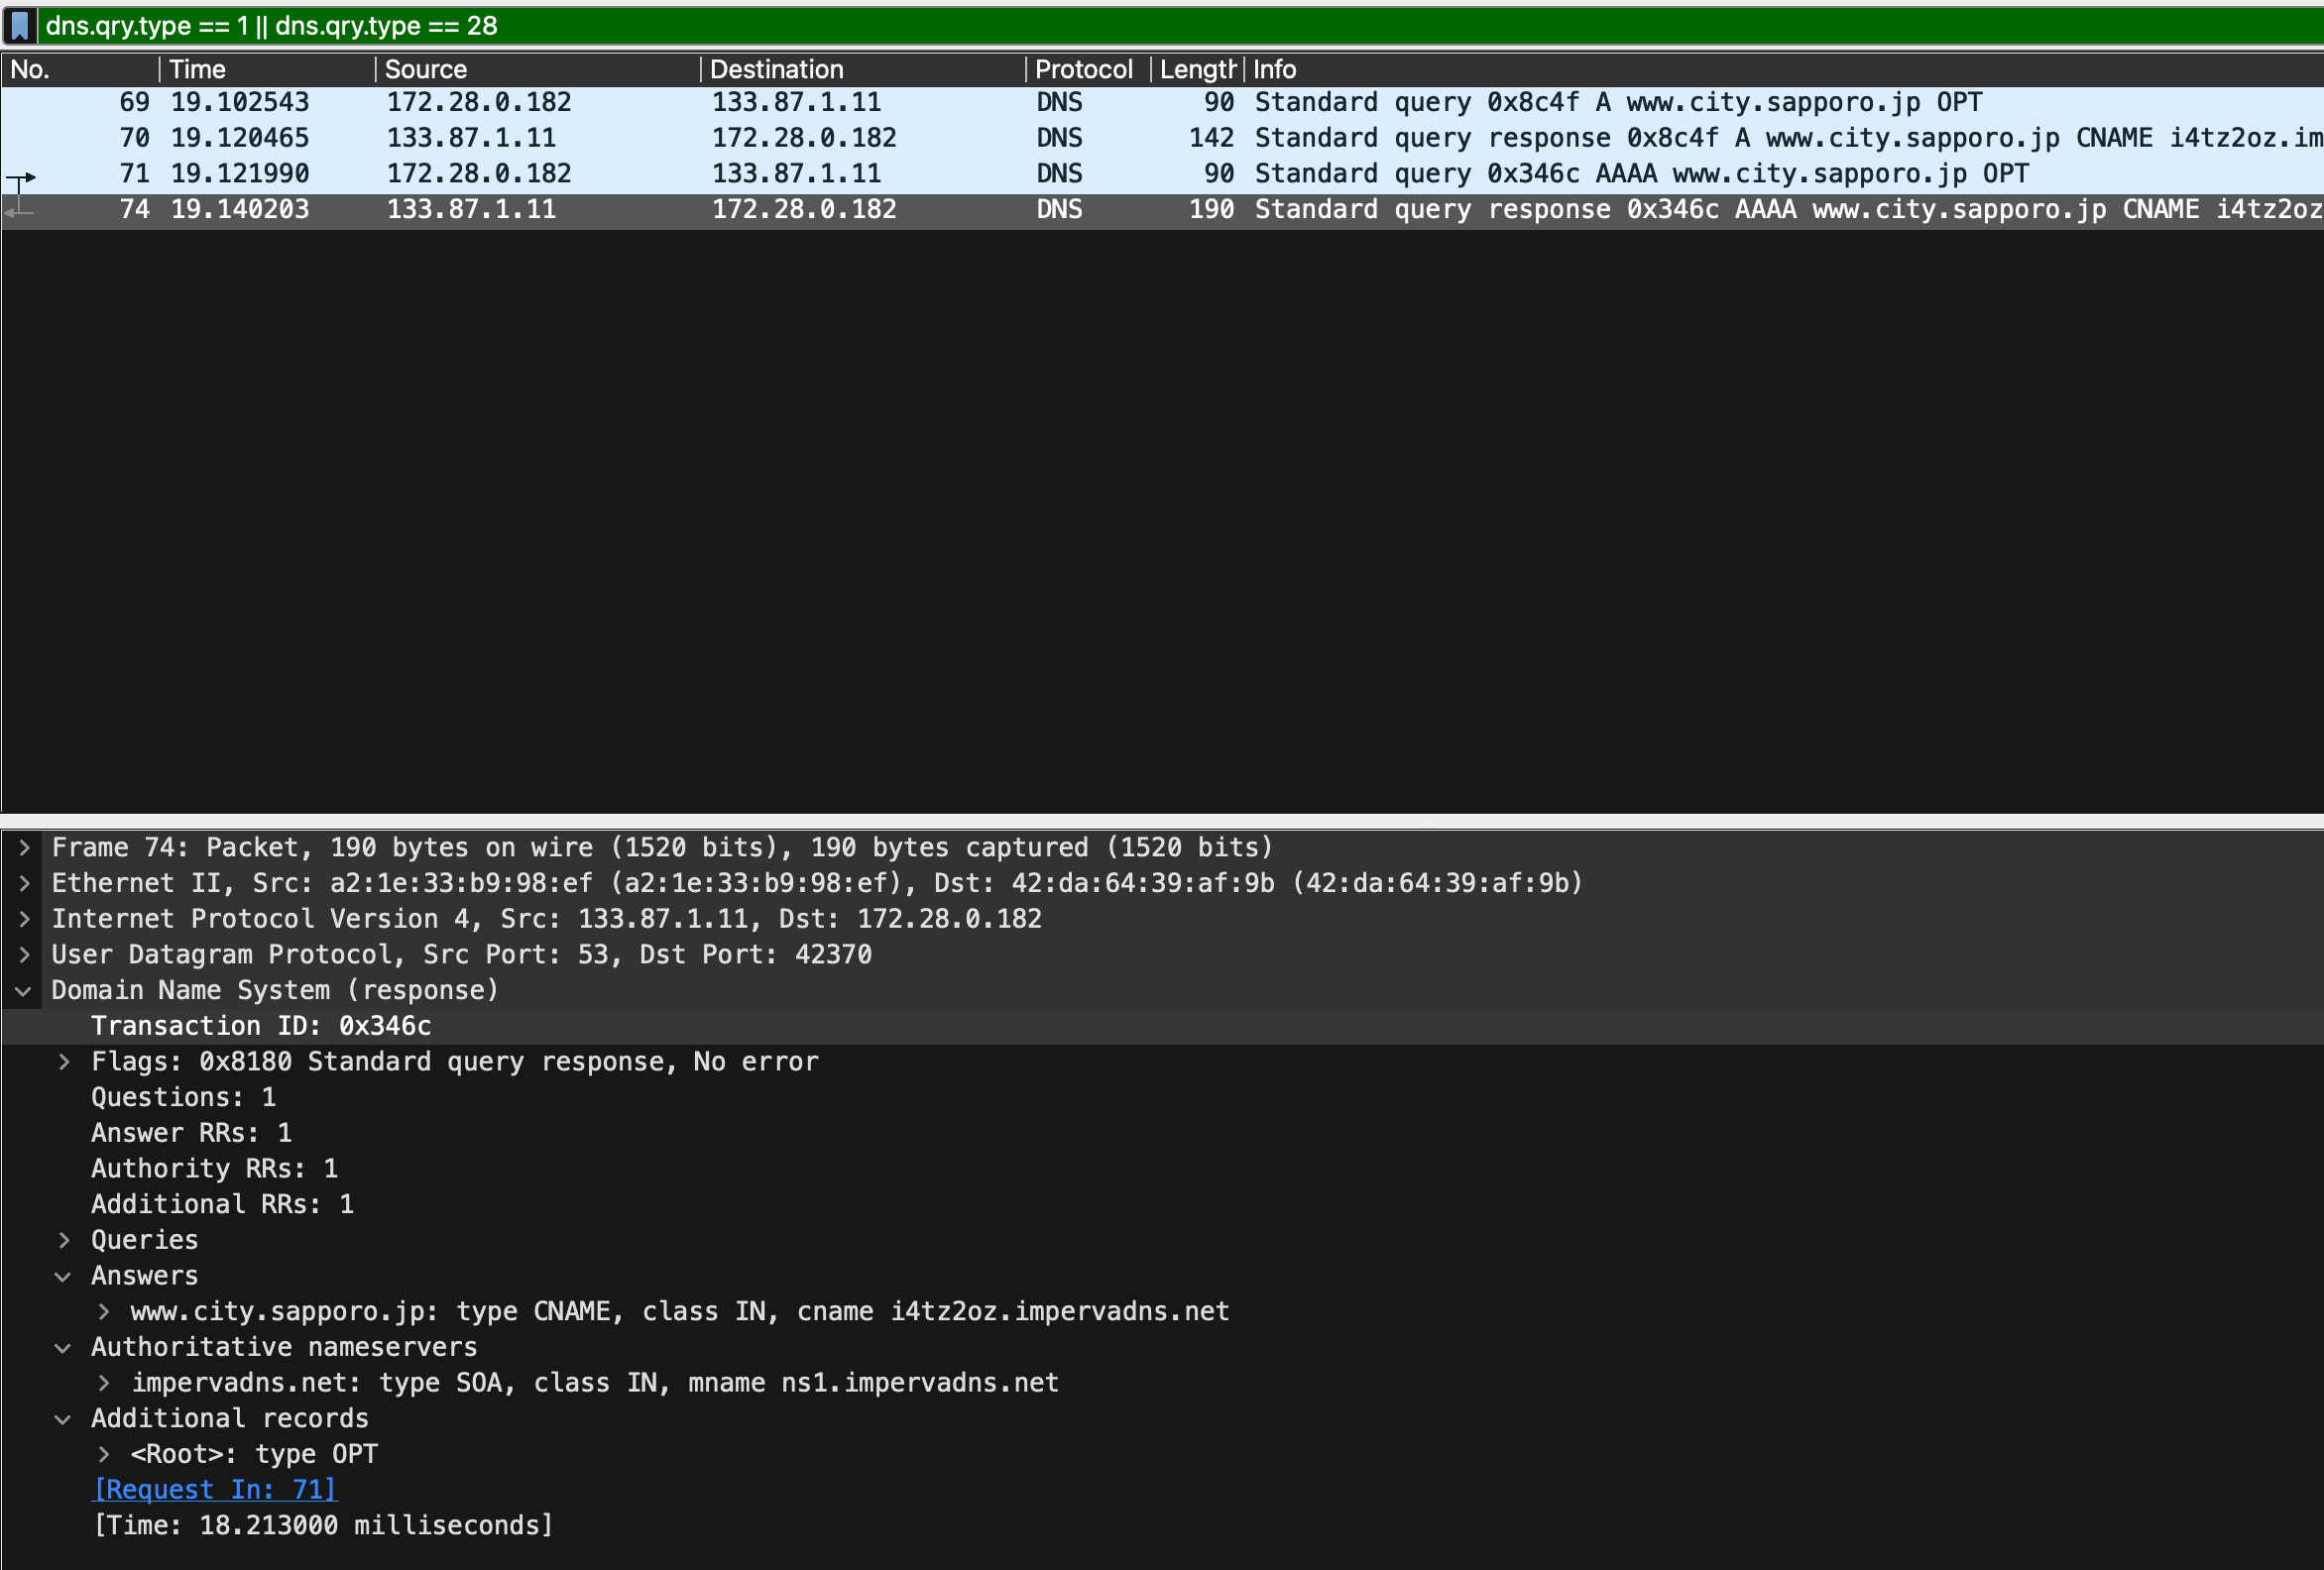
\includegraphics[width=0.98\columnwidth]{fig/wireshark_31_v4_answer.png}
    \caption{IPv4のみのホストのA・AAAAの応答}
    \label{fig:ws_31_v4_answer}
  \end{figure}

  \begin{figure}[h]
    \centering
    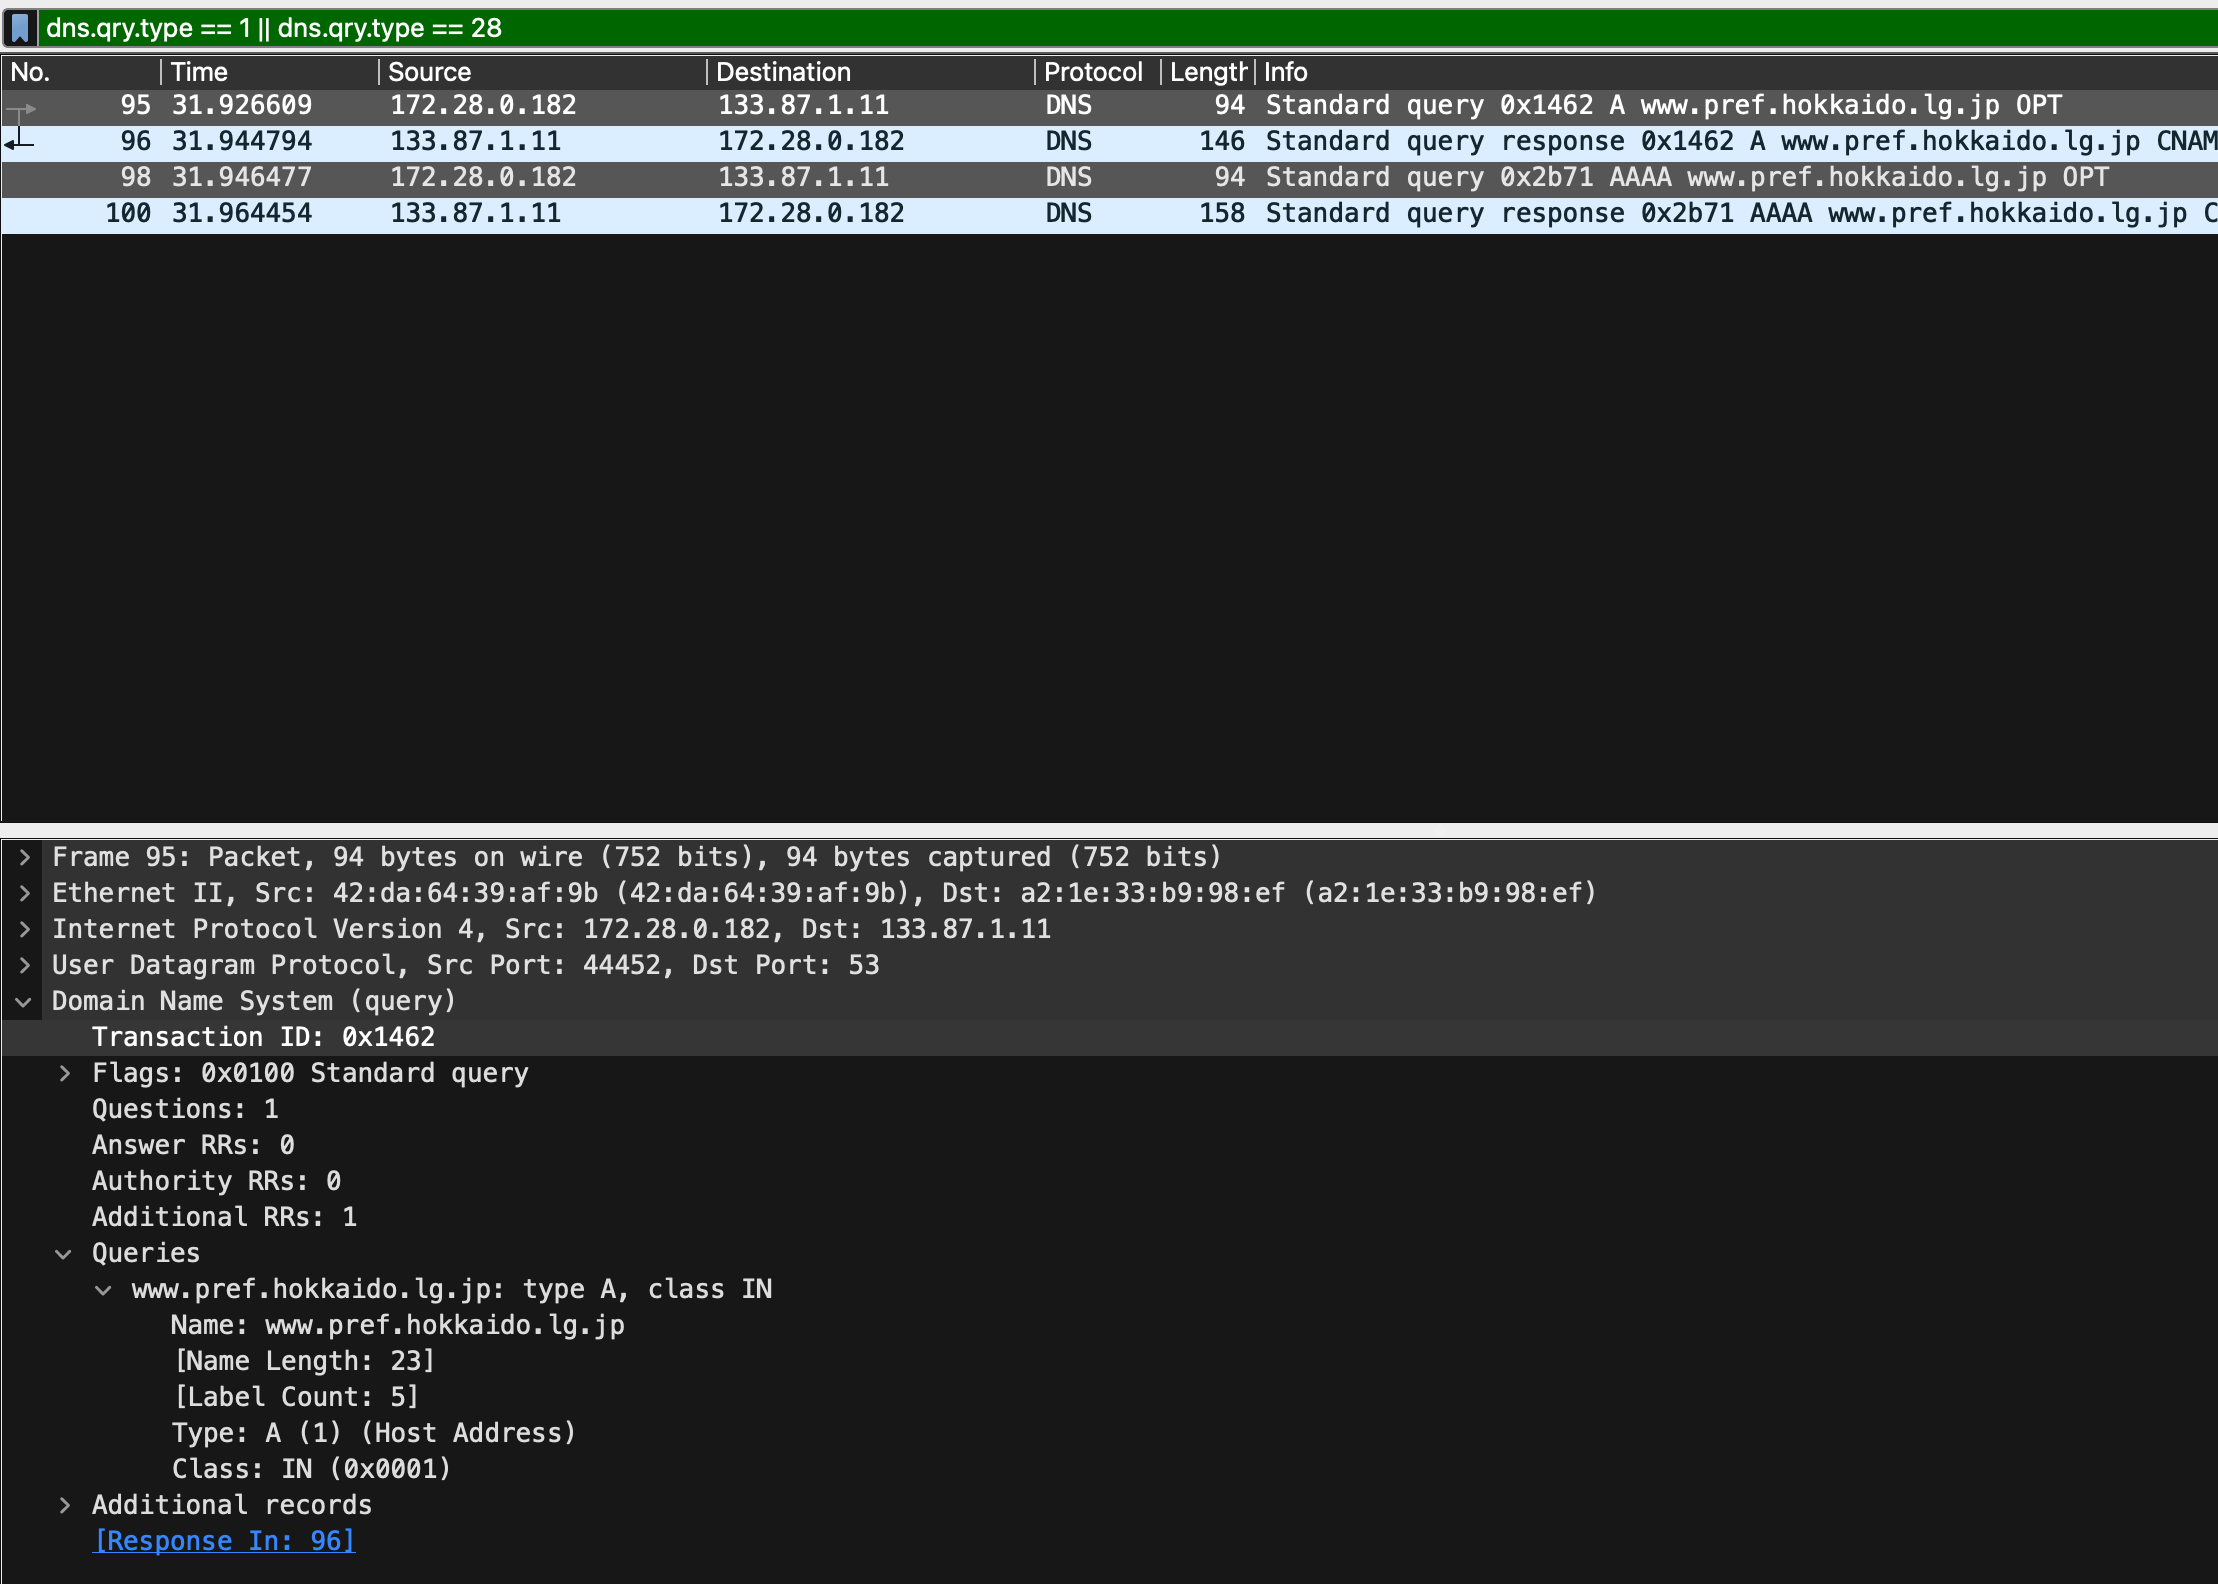
\includegraphics[width=0.98\columnwidth]{fig/wireshark_31_v46_query.png}
    \caption{両対応のホストのA・AAAAの問い合わせ}
    \label{fig:ws_31_v46_query}
  \end{figure}

  \begin{figure}[h]
    \centering
    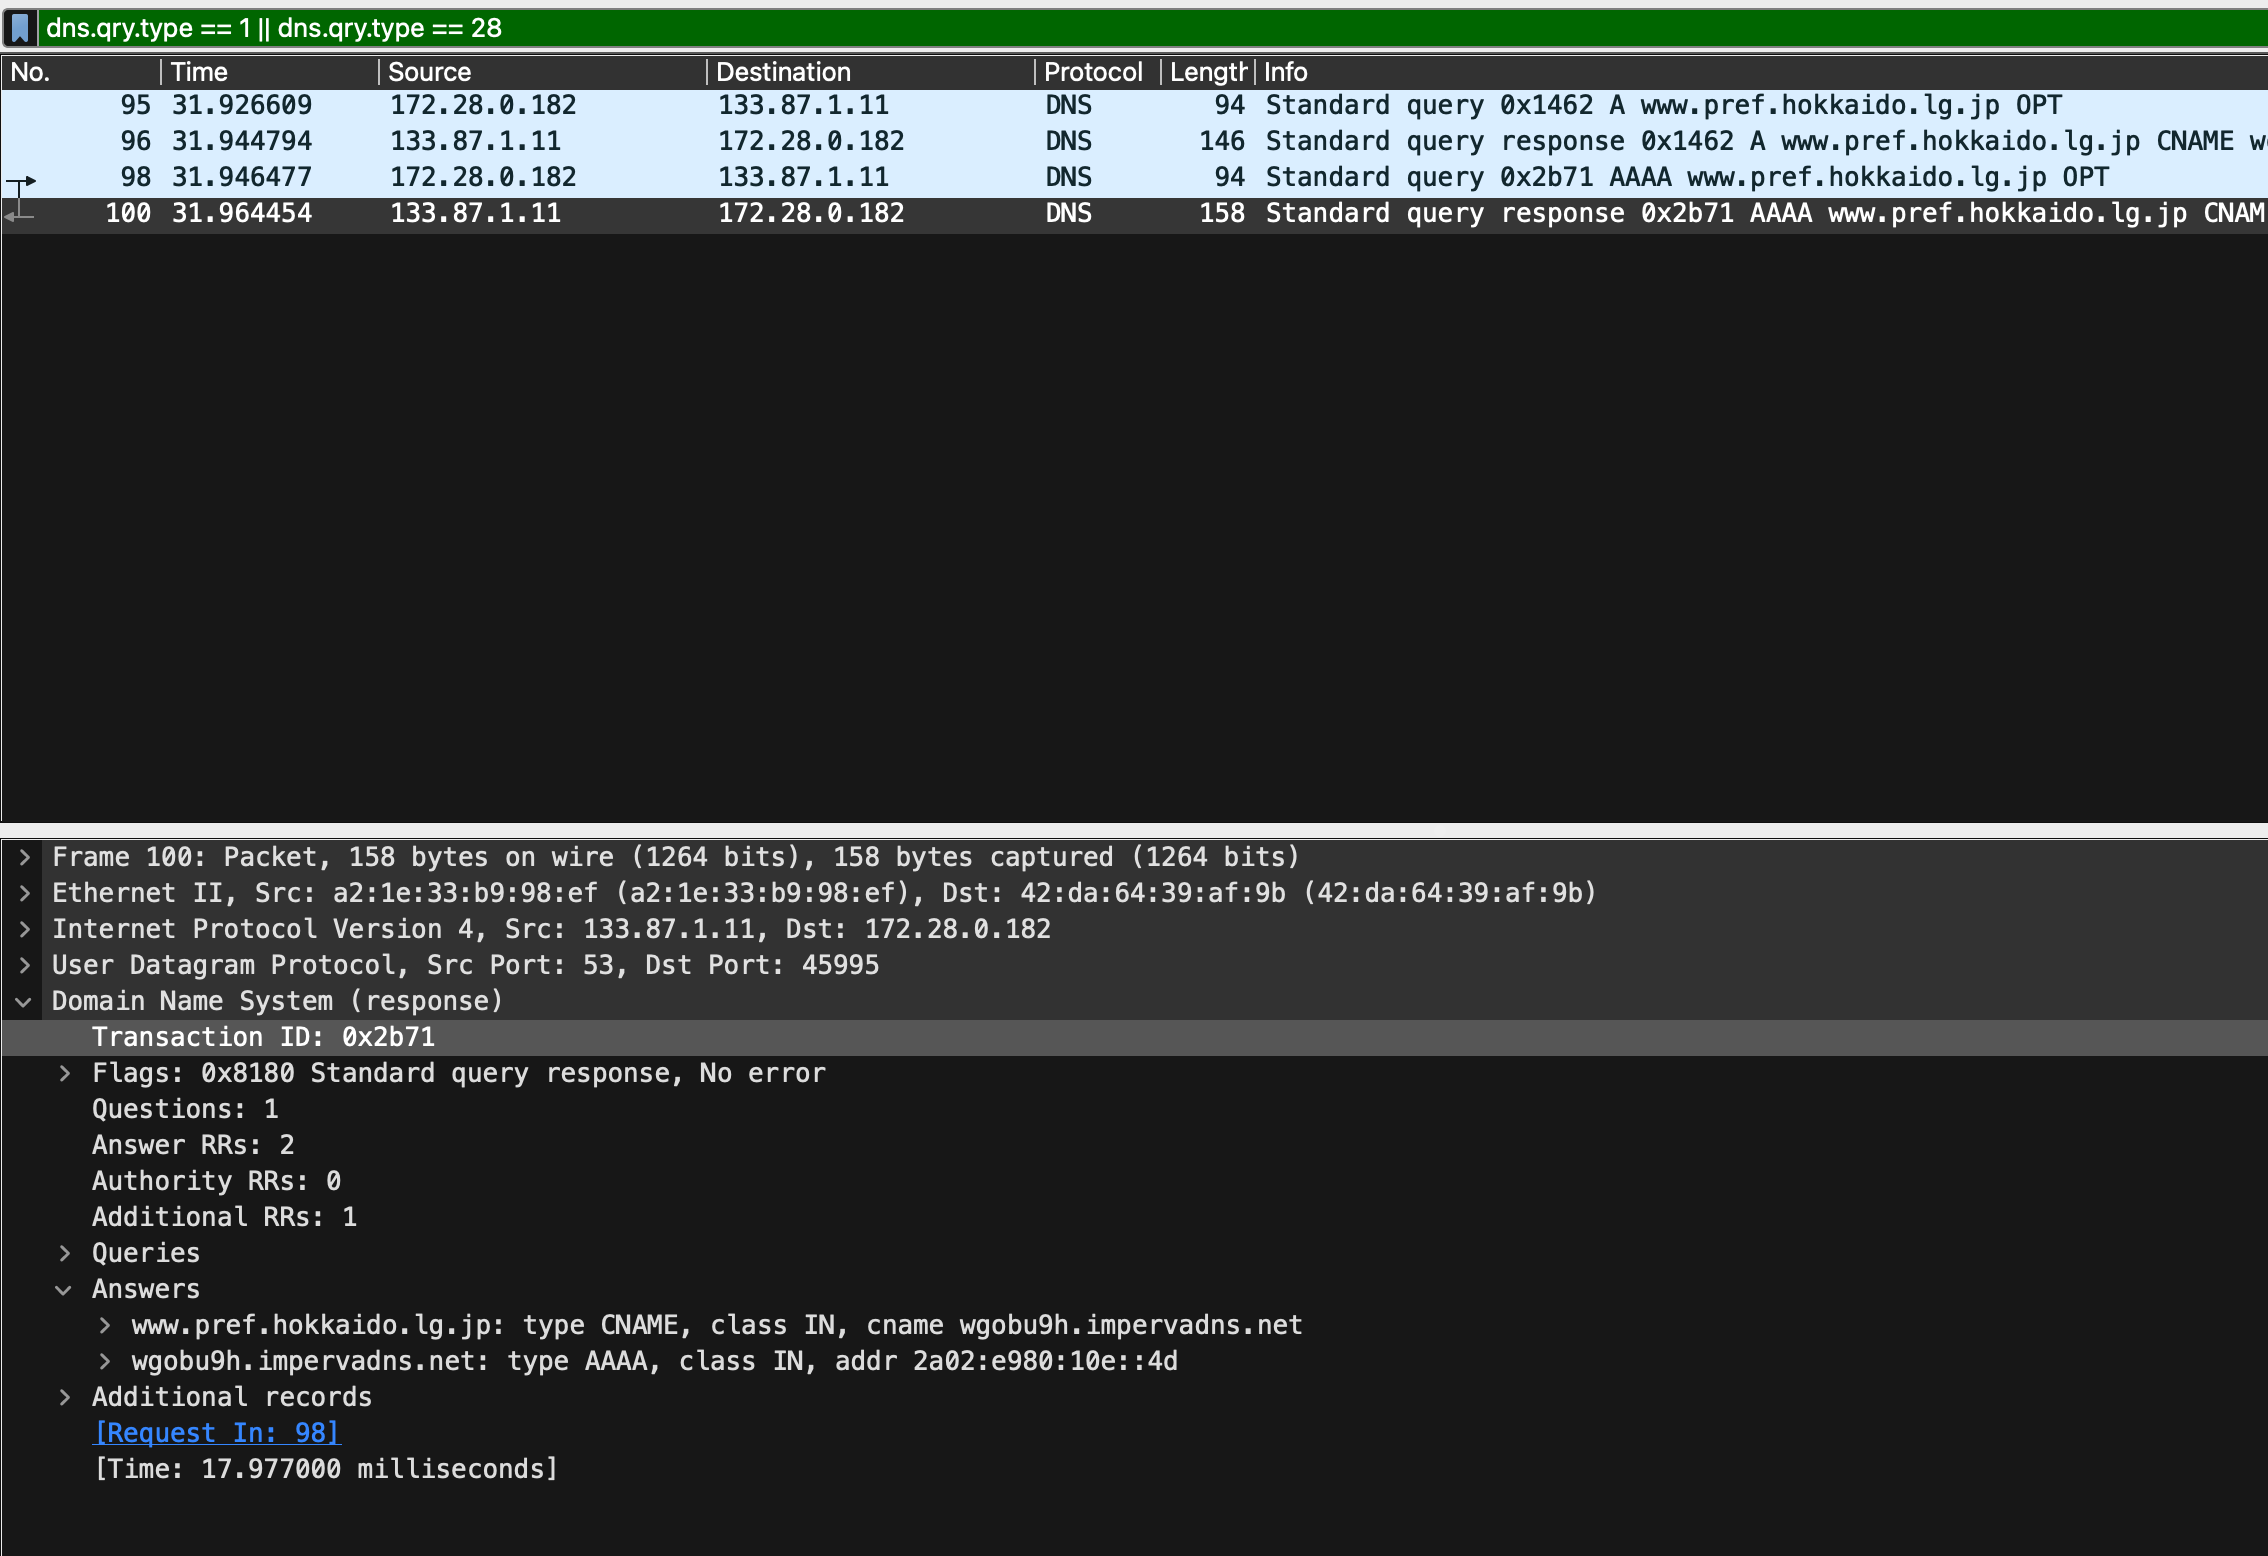
\includegraphics[width=0.98\columnwidth]{fig/wireshark_31_v46_answer.png}
    \caption{両対応のホストのA・AAAAの応答}
    \label{fig:ws_31_v46_answer}
  \end{figure}

  IPv4のみのホスト(www.city.sapporo.jp)では，図\ref{fig:ws_31_v4_query}のとおり，No.69でAレコード，No.71でAAAAレコードの問い合わせが，リゾルバ133.87.1.11(UDP 53番ポート)に送られた．図\ref{fig:ws_31_v4_answer}では，Aの応答(No.70)には，CNAME(i4tz2oz.impervadns.net)を経由してアドレス45.60.112.77(TTL 119秒)が含まれている一方，AAAAの応答(No.74)にはCNAMEとSOAのみが含まれ，AAAAレコードはなかった．これは，このホストがIPv6のアドレスを持たないことを示す．出力\ref{out:dnspy_v4}でも，Aレコードとして45.60.112.77が1件表示された一方，AAAAは``No answer from the resolver''と表示されており，パケットの内容と一致する．

  両対応のホスト(www.pref.hokkaido.lg.jp)では，図\ref{fig:ws_31_v46_query}のとおり，No.95でAレコード，No.98でAAAAレコードの問い合わせが同様にリゾルバ133.87.1.11に送られた．図\ref{fig:ws_31_v46_answer}では，Aの応答(No.96)にIPv4アドレス45.60.112.77(TTL 46秒)，AAAAの応答(No.100)にIPv6アドレス2a02:e980:10e::4d(TTL 46秒)が含まれた．どちらの応答にも，www.pref.hokkaido.lg.jpからwgobu9h.impervadns.netへのCNAMEが含まれ，その先のAレコード，AAAAレコードとしてアドレスが得られている．出力\ref{out:dnspy_v46}にも，同じ2つのアドレスが表示されている．

  2つのホストを比べると，どちらでもAとAAAAの2種類の問い合わせが同じリゾルバ(133.87.1.11)に送られており，問い合わせの手順は同じである．違いは応答の内容にあり，IPv4のみのホストではAAAAの応答にアドレスがなく，両対応のホストでは両方のアドレスが得られた．また，2つのホストのAレコードは，どちらも45.60.112.77と同じ値であった．これは，どちらのホストもimpervadns.net配下の名前へのCNAMEを経由しており(sapporoはi4tz2oz.impervadns.net，hokkaidoはwgobu9h.impervadns.net)，同じ事業者のサービス上に置かれているためと考えられる．また，AとAAAAの問い合わせは並行ではなく順に送られていた．Aの応答を受け取った約1.5ミリ秒後(No.70とNo.71の間)にAAAAの問い合わせが送られており，両対応のホストでも同様に，Aの応答(No.96)の約1.7ミリ秒後にAAAAの問い合わせ(No.98)が送られている．
\end{maintask}

  \begin{maintask}{3-2}
  \subsection*{課題内容}
  socketのgetaddrinfoで名前解決し，IPv4のみ対応のホストと両対応のホストで返るアドレスの違いを確認した．

  \subsection*{実験方法}
  \begin{enumerate}
    \item ホスト名を書き換えて実行（3-1と同じ2つのホスト）
      \begin{minted}{zsh}
        sed -i "s/^q_hostname = .*/q_hostname = 'www.city.sapporo.jp'/" dns_socket_sample.py
        ./dns_socket_sample.py
        sed -i "s/^q_hostname = .*/q_hostname = 'www.pref.hokkaido.lg.jp'/" dns_socket_sample.py
        ./dns_socket_sample.py
      \end{minted}
      出力に\texttt{AF\_INET}のみが並ぶか，\texttt{AF\_INET6}も並ぶかを比較した．
  \end{enumerate}

  \subsection*{結果}
  2つのホストに対する実行結果を，出力\ref{out:gai_v4}，出力\ref{out:gai_v46}に示した．使用したプログラムのソースコードをリスト\ref{lst:gai}に示す．\texttt{q\_hostname}の行は，ホスト名ごとに\texttt{sed}で書き換えて使用した．

  \begin{listing}[H]
    \caption{dns\_socket\_sample.py のソースコード}\label{lst:gai}
    \begin{minted}[fontsize=\small]{python}
    #!/usr/bin/python3

    import socket

    q_hostname = 'www.pref.hokkaido.lg.jp'

    print('Quering hostname:', q_hostname)

    addrs = socket.getaddrinfo(q_hostname, 443)
    for addr in addrs:
        print(addr)
    \end{minted}
  \end{listing}

  \begin{termout}[H]
    \caption{dns\_socket\_sample.py(www.city.sapporo.jp) の実行結果}\label{out:gai_v4}
    \begin{minted}{zsh}
    guest@host82:~/dns$ ./dns_socket_sample.py
    Quering hostname: www.city.sapporo.jp
    (<AddressFamily.AF_INET: 2>, <SocketKind.SOCK_STREAM: 1>, 6,
     '', ('45.60.112.77', 443))
    (<AddressFamily.AF_INET: 2>, <SocketKind.SOCK_DGRAM: 2>, 17,
     '', ('45.60.112.77', 443))
    (<AddressFamily.AF_INET: 2>, <SocketKind.SOCK_RAW: 3>, 0,
     '', ('45.60.112.77', 443))
    \end{minted}
  \end{termout}

  \begin{termout}[H]
    \caption{dns\_socket\_sample.py(www.pref.hokkaido.lg.jp) の実行結果}\label{out:gai_v46}
    \begin{minted}{zsh}
    guest@host82:~/dns$ ./dns_socket_sample.py
    Quering hostname: www.pref.hokkaido.lg.jp
    (<AddressFamily.AF_INET6: 10>, <SocketKind.SOCK_STREAM: 1>, 6,
     '', ('2a02:e980:10e::4d', 443, 0, 0))
    (<AddressFamily.AF_INET6: 10>, <SocketKind.SOCK_DGRAM: 2>, 17,
     '', ('2a02:e980:10e::4d', 443, 0, 0))
    (<AddressFamily.AF_INET6: 10>, <SocketKind.SOCK_RAW: 3>, 0,
     '', ('2a02:e980:10e::4d', 443, 0, 0))
    (<AddressFamily.AF_INET: 2>, <SocketKind.SOCK_STREAM: 1>, 6,
     '', ('45.60.112.77', 443))
    (<AddressFamily.AF_INET: 2>, <SocketKind.SOCK_DGRAM: 2>, 17,
     '', ('45.60.112.77', 443))
    (<AddressFamily.AF_INET: 2>, <SocketKind.SOCK_RAW: 3>, 0,
     '', ('45.60.112.77', 443))
    \end{minted}
  \end{termout}

  www.city.sapporo.jpでは，出力\ref{out:gai_v4}のとおり，返ってきたアドレスはすべて\texttt{AF\_INET}で，IPv4アドレス45.60.112.77(ポート443)だけが得られた．同じアドレスが3行並んでいるのは，ソケットの種類(\texttt{SOCK\_STREAM}，\texttt{SOCK\_DGRAM}，\texttt{SOCK\_RAW})ごとに1つずつ返されたためで，プロトコル番号はそれぞれ6(TCP)，17(UDP)，0である．これは3-1で，このホストのAAAAの応答にアドレスがなかったことと一致する．

  www.pref.hokkaido.lg.jpでは，出力\ref{out:gai_v46}のとおり，\texttt{AF\_INET6}のアドレス2a02:e980:10e::4dと，\texttt{AF\_INET}のアドレス45.60.112.77の両方が返った．各アドレスがソケットの種類ごとに3行ずつ並ぶ点は同じで，合計6行であった．また，\texttt{AF\_INET6}が先に並び，\texttt{AF\_INET}が後に続いた．getaddrinfoはRFC 6724に基づいて宛先アドレスを並べ替えるため，IPv6の優先度がIPv4より高く，IPv6が先頭になったと考えられる．実際，課題Eのwgetでも，www.pref.hokkaido.lg.jpへの接続にはIPv6が使われており，この順序と一致する．

  以上より，getaddrinfoは，DNSのAとAAAAの結果をまとめて返し，呼び出し側はそのアドレスファミリを見て接続先を選べる．ホストがIPv6に対応しているかどうかは，返るアドレスの種類で判断できる．
\end{maintask}

  \begin{maintask}{4-1}
  \subsection*{課題内容}
  UDPサーバ\texttt{udp\_server.py}とUDPクライアント\texttt{udp\_client.py}を実行し，クライアントから送信したデータをサーバが受信することを確認する．

  \subsection*{実験方法}
  \begin{enumerate}
    \item サンプルをホームディレクトリにコピーし，サーバを起動する．
      \begin{minted}{zsh}
        cd
        cp -r /shares/socket .
        cd socket
        ./udp_server.py
      \end{minted}
    \item 別の演習環境からクライアントを起動する．
      \begin{minted}{zsh}
        cd socket
        ./udp_client.py
      \end{minted}
    \item サーバ側とクライアント側の出力を確認し，サーバをCtrl-Cで停止する．
  \end{enumerate}

  \subsection*{結果}
  サーバ側とクライアント側の実行結果を出力\ref{out:udp_server}，出力\ref{out:udp_client}に示す．
  使用したソースコードをリスト\ref{lst:udp_server}，リスト\ref{lst:udp_client}に示す．
  \begin{listing}[H]
    \caption{udp\_server.py のソースコード}\label{lst:udp_server}
    \inputminted[fontsize=\small]{python}{src/day4/udp_server.py}
  \end{listing}
  \begin{listing}[H]
    \caption{udp\_client.py のソースコード}\label{lst:udp_client}
    \inputminted[fontsize=\small]{python}{src/day4/udp_client.py}
  \end{listing}
 
  \begin{termout}[H]
    \caption{udp\_server.py の実行結果}\label{out:udp_server}
    \begin{minted}{text}
    guest@host82:~/socket$ ./udp_server.py
    Starting the server at 2026-11-12 00:27:30.085333     
    Waiting for a client to call.                         
    At 2026-11-12 00:28:28.445504 ('127.0.0.1', 40714) said, Hey!  
    \end{minted}
  \end{termout}
  \begin{termout}[H]
    \caption{udp\_client.py の実行結果}\label{out:udp_client}
    \begin{minted}{text}
    guest@host82:~$ cd ~/socket
    guest@host82:~/socket$ ./udp_client.py                                                                        
    Staring the client at 2026-11-12 00:28:28.445191                                                              
    At 2026-11-12 00:28:28.445576 ('127.0.0.1', 6789) said, Are you talking to me?    
    \end{minted}
  \end{termout}

  クライアントが送信した\texttt{Hey!}をサーバが受信し，サーバからの応答\texttt{Are you talking to me?}をクライアントが受信した．UDPによる要求と応答が正常に行われた．
\end{maintask}

  \begin{maintask}{4-2}
  \subsection*{課題内容}
  \texttt{socket\_dns\_test.py}がDNS問い合わせに設定した乱数のQuery IDと，応答パケットのResponse IDが一致することを確認する．

  \subsection*{実験方法}
  \begin{enumerate}
    \item DNS問い合わせのパケットをキャプチャする．
      \begin{minted}{zsh}
        cd ~/socket
        tcpdump -i eth1 -s 0 -w day4_2_dns.pcap 'not port 4200'
      \end{minted}
    \item 別の端末でプログラムを実行する．引数には実際に問い合わせたホスト名を指定する．
      \begin{minted}{zsh}
        cd ~/socket
        ./socket_dns_test.py www.iic.hokudai.ac.jp
      \end{minted}
    \item キャプチャを停止し，pcapをWiresharkで開いてDNSのQueryとResponseを確認する．
  \end{enumerate}

  \subsection*{結果}
  プログラムの実行結果を出力\ref{out:dns_test}に示す．Wiresharkで確認したQuery IDとResponse IDを図\ref{fig:dns_id}に示す．
  使用した\texttt{socket\_dns\_test.py}のソースコードをリスト\ref{lst:dns_test_source}に示す．
  \begin{listing}[H]
    \caption{socket\_dns\_test.py のソースコード（1/4）}\label{lst:dns_test_source}
    \inputminted[fontsize=\scriptsize,firstline=1,lastline=33]{python}{src/day4/socket_dns_test.py}
  \end{listing}
  \begin{listing}[H]
    \caption{socket\_dns\_test.py のソースコード（2/4）}
    \inputminted[fontsize=\scriptsize,firstline=34,lastline=66]{python}{src/day4/socket_dns_test.py}
  \end{listing}
  \begin{listing}[H]
    \caption{socket\_dns\_test.py のソースコード（3/4）}
    \inputminted[fontsize=\scriptsize,firstline=67,lastline=99]{python}{src/day4/socket_dns_test.py}
  \end{listing}
  \begin{listing}[H]
    \caption{socket\_dns\_test.py のソースコード（4/4）}
    \inputminted[fontsize=\scriptsize,firstline=100,lastline=132]{python}{src/day4/socket_dns_test.py}
  \end{listing}

  \begin{termout}[H]
    \caption{socket\_dns\_test.py の実行結果}\label{out:dns_test}
    \begin{minted}{text}
    guest@host82:~/socket$ ./socket_dns_test.py www.iic.hokudai.ac.jp
    id = 52921                                                                                                    
    [(b'www.iic.hokudai.ac.jp', 1, 1, 86400, '133.50.42.161')]    
    \end{minted}
  \end{termout}
  \begin{figure}[H]
    \centering
    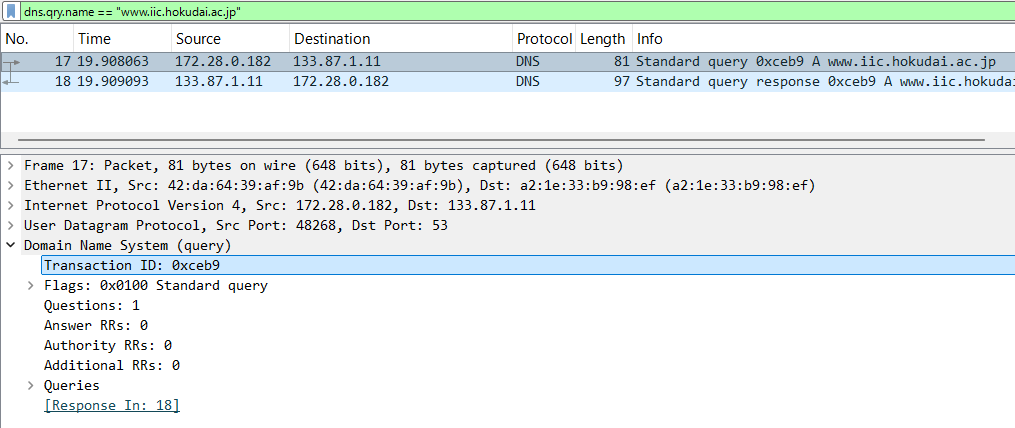
\includegraphics[width=0.98\columnwidth]{fig/wireshark_day4_2_dns_id.png}
    \caption{DNS Query IDとResponse IDの確認}\label{fig:dns_id}
  \end{figure}

  プログラムが表示したIDは10進数で52921，16進数で\texttt{0xceb9}であった．WiresharkでもQueryとResponseのTransaction IDはいずれも\texttt{0xceb9}であり，問い合わせと応答のIDが一致した．
\end{maintask}

  \begin{extask}{4-3}
  \subsection*{課題内容}
  \texttt{socket\_dns\_test.py}が生成したDNS問い合わせパケットの内容を確認し，DNSの規定に沿っているかを調べる．

  \subsection*{実験方法}
  \begin{enumerate}
    \item 4-2で取得したpcapをWiresharkで開き，DNS Queryパケットを選択する．
    \item DNSヘッダとQuestionセクションを展開し，ID，フラグ，質問数，問い合わせ名，問い合わせ型，クラスを確認する．
    \item 指導書で指定されたDNS形式・RFCの記述と照合する．
  \end{enumerate}

  \subsection*{結果}
  DNS問い合わせパケットの画面を図\ref{fig:dns_format}に示す．
  \begin{figure}[H]
    \centering
    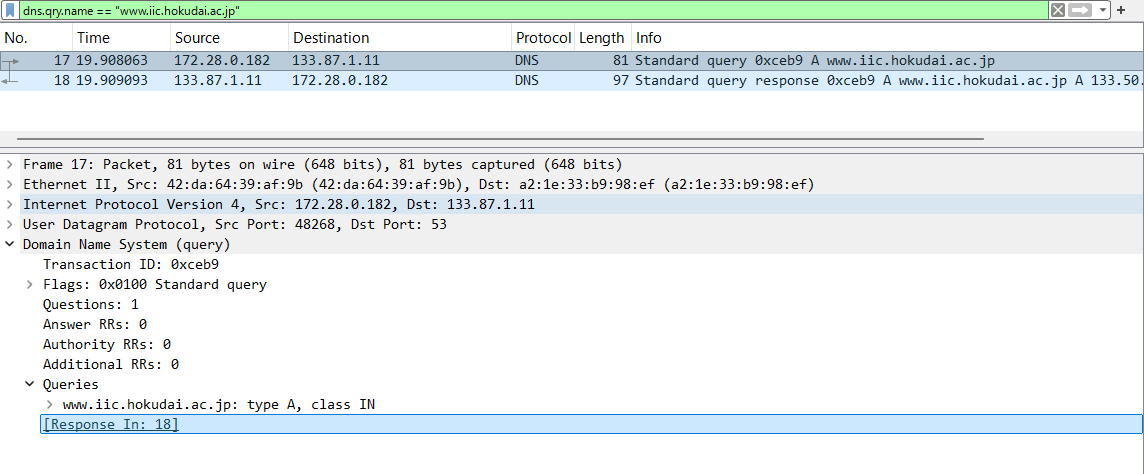
\includegraphics[width=0.98\columnwidth]{fig/wireshark_day4_3_dns_format.png}
    \par\smallskip
    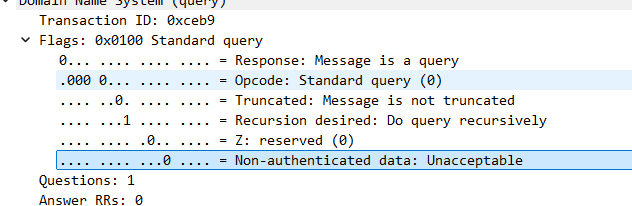
\includegraphics[width=0.72\columnwidth]{fig/wireshark_day4_3_dns_flags.png}
    \par\smallskip
    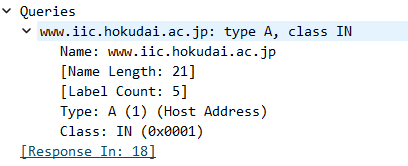
\includegraphics[width=0.72\columnwidth]{fig/wireshark_day4_3_dns_question.png}
    \caption{DNS問い合わせパケットの構造}\label{fig:dns_format}
  \end{figure}

  Wiresharkで確認したTransaction IDは\texttt{0xceb9}，Flagsは\texttt{0x0100}，Questionsは1であり，Answer/Authority/Additional RRsはいずれも0であった．Flagsの内訳は，QR=0（問い合わせ），Opcode=0（標準問い合わせ），TC=0（切り詰めなし），RD=1（再帰問い合わせ希望），予約ビット=0，AD=0であった．ADビットを問い合わせでクリアする形式はRFC 4035 §4.6にも沿っている．QuestionはQNAME=\texttt{www.iic.hokudai.ac.jp}，QTYPE=A（1），QCLASS=IN（\texttt{0x0001}）である．DNSヘッダおよび質問部の形式を定めるRFC 1035 §4.1.1–4.1.2と照合し，確認した値は標準問い合わせの形式に沿っていることを確認した．
\end{extask}

  \begin{maintask}{4-4}
  \subsection*{課題内容}
  TCPサーバ\texttt{tcp\_server.py}とTCPクライアント\texttt{tcp\_client.py}を実行し，クライアントから送信した文字列をサーバが受信することを確認する．

  \subsection*{実験方法}
  \begin{enumerate}
    \item サンプルをコピーした\texttt{~/socket}で，サーバの接続先をsshdのIPv4またはIPv6アドレスに設定して起動する．
      \begin{minted}{zsh}
        cd ~/socket
        ./tcp_server.py
      \end{minted}
    \item 別の演習環境で\texttt{tcp\_client.py}を実行し，メッセージを送る．
      \begin{minted}{zsh}
        cd ~/socket
        ./tcp_client.py
      \end{minted}
    \item サーバ側で受信した文字列と接続元を確認し，サーバをCtrl-Cで停止する．
  \end{enumerate}

  \subsection*{結果}
  サーバ側・クライアント側の実行結果を出力\ref{out:tcp_server}，出力\ref{out:tcp_client}に示す．
  使用したサーバのソースコードをリスト\ref{lst:tcp_server_44}に示す．
  \begin{listing}[H]
    \caption{tcp\_server.py のソースコード}\label{lst:tcp_server_44}
    \inputminted[fontsize=\small]{python}{src/day4/tcp_server.py}
  \end{listing}
  \begin{listing}[H]
    \caption{4-4で使用したIPv4版tcp\_client.py}\label{lst:tcp_client_44}
    \begin{minted}[fontsize=\small]{python}
    #!/usr/bin/python3
    from datetime import datetime
    import socket

    HOSTNAME = '127.0.0.1'
    PORT_NUM = 6789
    MAX_SIZE = 1024

    print('The client started at', datetime.now())
    with socket.socket(socket.AF_INET, socket.SOCK_STREAM) as server:
        server.connect((HOSTNAME, PORT_NUM))
        print("Input text: ", end='')
        msg = input()
        server.sendall(msg.encode('utf-8'))
        data = server.recv(MAX_SIZE)
        print('Echo back text:', data.decode('utf-8'))
    \end{minted}
  \end{listing}
  \begin{termout}[H]
    \caption{tcp\_server.py の実行結果}\label{out:tcp_server}
    \begin{minted}{text}
    guest@host82:~/socket$ ./tcp_server.py
    The server started at 2026-11-12 00:40:38.153942
    Waiting...
    Received text: Test message. from  ('127.0.0.1', 55982)
    \end{minted}
  \end{termout}
  \begin{termout}[H]
    \caption{tcp\_client.py の実行結果}\label{out:tcp_client}
    \begin{minted}{text}
    guest@host82:~/socket$ ./tcp_client.py                                                                        
    The client started at 2026-11-12 00:42:33.305380                                                              
    Input text: Test message.                                                                                     
    Echo back text: Test message.   
    \end{minted}
  \end{termout}

  クライアントが送信した\texttt{Test message.}をサーバが受信し，同じ文字列がクライアントにも返された．
\end{maintask}

  \begin{maintask}{4-5}
  \subsection*{課題内容}
  \texttt{tcp\_client.py}の接続先を172.28.0.200，サービスをecho (TCPポート7)に変更し，送信した文字列が返ることを確認する．

  \subsection*{実験方法}
  \begin{enumerate}
    \item \texttt{tcp\_client.py}の接続先を172.28.0.200，ポートをecho (7/tcp)に変更する．
    \item プログラムを実行し，入力文字列とエコーされた文字列を記録する．
  \end{enumerate}

  \subsection*{結果}
  実行に用いた\texttt{tcp\_client.py}のソースコードをリスト\ref{lst:tcp_echo_client}に，実行結果を出力\ref{out:tcp_echo_client}に示す．
  \begin{listing}[H]
    \caption{echoサーバ向けtcp\_client.py のソースコード}\label{lst:tcp_echo_client}
    \begin{minted}[fontsize=\small]{python}
    #!/usr/bin/python3

    from datetime import datetime
    import socket
                                                                                                                  
                                                                                                                  
    #HOSTNAME = '::1'
    HOSTNAME = '172.28.0.200'
    PORT_NUM = 7
                                                                                                                  
    MAX_SIZE= 1024
                                                                                                                  
    print('The client started at', datetime.now())
                                                                                                                  
                                                                                                                  
    # 1. socketの作成
    # IPv4 の場合は AF_INETの行を有効化し、v6の場合はAF_INET6の行を有効化する
    with socket.socket(socket.AF_INET, socket.SOCK_STREAM) as server:
    #with socket.socket(socket.AF_INET6, socket.SOCK_STREAM) as server:
    # 2. ソケットのサーバへの接続 (connect)
    server.connect((HOSTNAME, PORT_NUM))                                                                      
    print("Input text: ", end='')
    msg = input()
    # 3. メッセージの送受信 (sendall, recv)
    server.sendall(msg.encode('utf-8'))
    data = server.recv(MAX_SIZE)                                                                              
    print('Echo back text:', data.decode('utf-8'))
    server.close()          
    \end{minted}
  \end{listing}
  \begin{termout}[H]
    \caption{echoサーバとの通信結果}\label{out:tcp_echo_client}
    \begin{minted}{text}
    guest@host82:~/socket$ ./tcp_client.py
    The client started at 2026-11-12 00:59:51.087378
    Input text: Hello World.
    Echo back text: Hello World.
    \end{minted}
  \end{termout}

  接続先を\texttt{172.28.0.200:7}に設定し，\texttt{Hello World.}を送信したところ，同じ文字列が返された．
\end{maintask}

  \begin{maintask}{4-6}

  \subsection*{課題内容}
  \texttt{tcp\_client.py}の接続先を172.28.0.200のTCPポート6789に変更し，サーバが混雑しているときにすぐ返事が返らないことを確認する．

  \subsection*{実験方法}
  \begin{enumerate}
    \item 接続先を172.28.0.200，ポートを6789に変更した\texttt{tcp\_client.py}を実行する．
    \item 応答が返るまでの様子を記録し，演習環境の指示に従って終了する．
  \end{enumerate}

  \subsection*{結果}
  使用したソースコードをリスト\ref{lst:tcp_busy_client}に，実行結果を出力\ref{out:tcp_busy_client}に示す．
  \begin{listing}[H]
    \caption{混雑時の確認に用いたtcp\_client.py}\label{lst:tcp_busy_client}
    \begin{minted}[fontsize=\small]{python}
    #!/usr/bin/python3

    from datetime import datetime
    import socket
                                                                                                              
                                                                                                              
    #HOSTNAME = '::1'
    HOSTNAME = '172.28.0.200'
    PORT_NUM = 6789
                                                                                                              
    MAX_SIZE= 1024
                                                                                                              
    print('The client started at', datetime.now())
                                                                                                              
                                                                                                              
    # 1. socketの作成
    # IPv4 の場合は AF_INETの行を有効化し、v6の場合はAF_INET6の行を有効化する
    with socket.socket(socket.AF_INET, socket.SOCK_STREAM) as server:
    #with socket.socket(socket.AF_INET6, socket.SOCK_STREAM) as server:
    # 2. ソケットのサーバへの接続 (connect)
    server.connect((HOSTNAME, PORT_NUM))                                                                      
    print("Input text: ", end='')
    msg = input()
    # 3. メッセージの送受信 (sendall, recv)
    server.sendall(msg.encode('utf-8'))
    data = server.recv(MAX_SIZE)                                                                              
    print('Echo back text:', data.decode('utf-8'))
    server.close()                                                                                            
                          
    \end{minted}
  \end{listing}
  \begin{termout}[H]
    \caption{TCPポート6789への接続結果}\label{out:tcp_busy_client}
    \begin{minted}{text}
    guest@host82:~/socket$ ./tcp_client.py                                                                        
    The client started at 2026-11-12 01:04:07.031393                                                              
    Input text: Hello message.                                                                                    
    Echo back text: Hello message.     
    \end{minted}
  \end{termout}

  接続先\texttt{172.28.0.200:6789}に\texttt{Hello message.}を送信し，\texttt{Hello message.}が返ることを確認した．記録された出力には応答までの待ち時間が含まれていないため，応答遅延の程度はこのログからは評価できない．
\end{maintask}

  \begin{maintask}{4-7}
  \subsection*{課題内容}
  IPv6対応の3種類のTCPサーバ（select，fork，multithreading）を起動し，IPv6対応クライアントから接続できることを確認する．

  \subsection*{実験方法}
  \begin{enumerate}
    \item 各サーバプログラムを\texttt{~/socket}で順番に起動する．
    \item クライアントをIPv6対応にし，サーバのIPv6アドレスに接続してメッセージを送信する．
    \item サーバごとにクライアントとサーバ両方の出力を記録し，次のサーバを試す前に停止する．
  \end{enumerate}

  \subsection*{結果}
  各サーバに対するクライアント・サーバの実行結果を出力\ref{out:select_server}〜出力\ref{out:thread_client}に示す．使用したソースコードをリスト\ref{lst:select_server}〜リスト\ref{lst:ipv6_client}に示す．

  \begin{listing}[H]
    \caption{IPv6対応tcp\_server\_select.py}\label{lst:select_server}
    \begin{minted}[fontsize=\small]{python}
    #!/usr/bin/python3

    from datetime import datetime
    import socket
    import select
    import sys

    HOSTNAME = ''
    PORT_NUM = 6789
    MAX_SIZE = 1024

    print('The server started at', datetime.now())
    print('Waiting...')

    def accept_loop(server_sock):
      fds = [server_sock]
      while True:
        r, _, _ = select.select(fds, [], [])
        for sock in r:
          if sock == server_sock:
            new_sock, addr = sock.accept()
            fds.append(new_sock)
          else:
            data = sock.recv(MAX_SIZE)
            if not data:
              break
            print('Received text:', data.decode('utf-8'), 'from', addr)
            sock.sendall(data)
            sock.close()
            fds.remove(sock)

    if __name__ == '__main__':
      server = socket.socket(socket.AF_INET6, socket.SOCK_STREAM)
      #server = socket.socket(socket.AF_INET, socket.SOCK_STREAM)
      server.bind((HOSTNAME, PORT_NUM))
      server.listen()
      try:
        accept_loop(server)
      except KeyboardInterrupt:
        server.close()
    \end{minted}
  \end{listing}
  \begin{listing}[H]
    \caption{IPv6対応tcp\_server\_fork.py}\label{lst:fork_server}
    \begin{minted}[fontsize=\small]{python}
    #!/usr/bin/python3

    from datetime import datetime
    import socket
    import os

    HOSTNAME = ''
    PORT_NUM = 6789
    MAX_SIZE = 1024

    print('The server started at', datetime.now())
    print('Waiting...')

    #with socket.socket(socket.AF_INET, socket.SOCK_STREAM) as server:
    with socket.socket(socket.AF_INET6, socket.SOCK_STREAM) as server:
      server.bind((HOSTNAME, PORT_NUM))
      server.listen()
      try:
        while True:
          client, addr = server.accept()
          child_pid = os.fork()
          if child_pid == 0:
            data = client.recv(MAX_SIZE)
            if data:
              print('Received text:', data.decode('utf-8'), 'from', addr)
              client.sendall(data)
              client.close()
      except KeyboardInterrupt:
        pass
    \end{minted}
  \end{listing}
  \begin{listing}[H]
    \caption{IPv6対応tcp\_server\_multithreading.py}\label{lst:thread_server}
    \begin{minted}[fontsize=\small]{python}
    #!/usr/bin/python3

    from datetime import datetime
    import socket
    import threading

    alive = True
    observe_thread = None
    HOSTNAME = ''
    PORT_NUM = 6789
    MAX_SIZE = 1024

    print('The server started at', datetime.now())
    print('Waiting...')

    def client_handler(client, addr):
      data = client.recv(MAX_SIZE)
      if data:
        print('Received text:', data.decode('utf-8'), 'from', addr)
        client.sendall(data)
        client.close()

    if __name__ == '__main__':
      #with socket.socket(socket.AF_INET, socket.SOCK_STREAM) as server:
      with socket.socket(socket.AF_INET6, socket.SOCK_STREAM) as server:
        server.bind((HOSTNAME, PORT_NUM))
        server.listen()
        try:
          while True:
            client, addr = server.accept()
            thread = threading.Thread(target = client_handler, args = (client, addr))
            thread.start()
            while thread.is_alive():
              thread.join()
        except KeyboardInterrupt:
          alive = False
          pass
    \end{minted}
  \end{listing}
  \begin{listing}[H]
    \caption{IPv6対応tcp\_client.py}\label{lst:ipv6_client}
    \begin{minted}[fontsize=\small]{python}
    #!/usr/bin/python3

    from datetime import datetime
    import socket

    HOSTNAME = '::1'
    #HOSTNAME = '172.28.0.200'
    PORT_NUM = 6789
    MAX_SIZE= 1024

    print('The client started at', datetime.now())

    #with socket.socket(socket.AF_INET, socket.SOCK_STREAM) as server:
    with socket.socket(socket.AF_INET6, socket.SOCK_STREAM) as server:
        server.connect((HOSTNAME, PORT_NUM))
        print("Input text: ", end='')
        msg = input()
        server.sendall(msg.encode('utf-8'))
        data = server.recv(MAX_SIZE)
        print('Echo back text:', data.decode('utf-8'))
        server.close()
    \end{minted}
  \end{listing}

  \begin{termout}[H]
    \caption{selectサーバの実行結果}\label{out:select_server}
    \begin{minted}{text}
    guest@host82:~/socket$ ./tcp_server_select.py
    The server started at 2026-11-12 01:11:10.323441
    Waiting...
    Received text: How are you doing. from ('::1', 41992, 0, 0)
    guest@host82:~/socket$ ./tcp_client.py
    The client started at 2026-11-12 01:11:31.124926
    Input text: How are you doing.
    Echo back text: How are you doing.
    \end{minted}
  \end{termout}
  \begin{termout}[H]
    \caption{forkサーバの実行結果}\label{out:fork_server}
    \begin{minted}{text}
    guest@host82:~/socket$ ./tcp_server_fork.py
    The server started at 2026-11-12 01:16:08.792394
    Waiting...
    Received text: Text. from ('::1', 39216, 0, 0)
    guest@host82:~/socket$ ./tcp_client.py
    The client started at 2026-11-12 01:16:30.536484
    Input text: Text.
    Echo back text: Text.
    \end{minted}
  \end{termout}
  \begin{termout}[H]
    \caption{multithreadingサーバの実行結果}\label{out:thread_client}
    \begin{minted}{text}
    guest@host82:~/socket$ ./tcp_server_multithreading.py
    The server started at 2026-11-12 01:25:56.407150
    Waiting...
    Received text: Test message. from ('::1', 43042, 0, 0)
    guest@host82:~/socket$ ./tcp_client.py
    The client started at 2026-11-12 01:26:39.304585
    Input text: Test message.
    Echo back text: Test message.
    \end{minted}
  \end{termout}

  IPv6ループバック\texttt{::1}を用いて3種類のサーバに接続した．selectサーバでは\texttt{How are you doing.}，forkサーバでは\texttt{Text.}，multithreadingサーバでは\texttt{Test message.}を送信し，それぞれ同じ文字列がクライアントに返り，サーバ側にも接続元\texttt{::1}と受信文字列が表示された．
\end{maintask}

  \begin{maintask}{4-8}
  \subsection*{課題内容}
  \texttt{tcp\_server\_fork.py}の実行中に\texttt{ps}コマンドでプロセス一覧を確認し，クライアント接続時にプロセス数が増えることを確かめる．

  \subsection*{実験方法}
  \begin{enumerate}
    \item IPv6対応に変更した\texttt{tcp\_server\_fork.py}を起動し，クライアントから接続する．
    \item クライアントとの通信後，別端末から\texttt{ps}を実行してサーバの親子プロセスを確認する．
  \end{enumerate}

  \subsection*{結果}
  クライアントとの通信後に実行した\texttt{ps}の出力を出力\ref{out:ps_after}に示す．
  \begin{termout}[H]
    \caption{クライアント接続後のプロセス一覧}\label{out:ps_after}
    \begin{minted}{text}
    guest@host82:~/socket$ ps -ef | grep tcp_server_fork.py
    guest       1746    1676  0 01:16 pts/0    00:00:00 /usr/bin/python3 ./tcp_server_fork.py
    guest       1748    1746  0 01:16 pts/0    00:00:00 /usr/bin/python3 ./tcp_server_fork.py
    guest       1750    1703  0 01:24 pts/1    00:00:00 grep --color=auto tcp_server_fork.py
    \end{minted}
  \end{termout}

  クライアント接続後のプロセス一覧では，PID 1746のサーバプロセスに加えて，その子プロセスPID 1748が確認できた．子プロセスのPPIDは1746であり，クライアント接続を処理するためにforkで子プロセスが生成されたことが分かる．接続前の一覧は記録していないため，ここでは接続後の親子関係を示した．
\end{maintask}

  % \begin{maintask}{F}
  \subsection*{課題内容}
  HTTP/3対応のWebサイトにcurlでアクセスし，通信をキャプチャしてHTTP/2と比較した．

  \subsection*{実験方法}
  \begin{enumerate}
    \item HTTP/3でアクセスし，ヘッダを取得
      \begin{minted}{zsh}
        tcpdump -i eth1 -s 0 -w day2_F_h3.pcap 'not port 4200'    (1つ目のターミナル)
        curl -I --http3 https://www.cloudflare.com                (2つ目のターミナル)
      \end{minted}

    \item 比較用にHTTP/2でアクセス
      \begin{minted}{zsh}
        tcpdump -i eth1 -s 0 -w day2_F_h2.pcap 'not port 4200'    (1つ目のターミナル)
        curl -I --http2 https://www.cloudflare.com                (2つ目のターミナル)
      \end{minted}

    \item 表にないHTTP/3対応サイトの探索．alt-svcヘッダにh3が含まれるサイトを探す
      \begin{minted}{zsh}
        curl -sI https://<候補のURL> | grep -i alt-svc
      \end{minted}

    \item 各pcapをWiresharkで開き，次のフィルタを適用
      \begin{minted}{text}
        (HTTP/3) quic
        (HTTP/2) tcp.port == 443
      \end{minted}
  \end{enumerate}

  \subsection*{結果}
  HTTP/3・HTTP/2それぞれのtcpdumpとcurlの実行結果を出力\ref{out:f_h3}，出力\ref{out:f_h2}に，alt-svcの探索結果を出力\ref{out:f_altsvc}に示した．

  \begin{termout}[H]
    \caption{HTTP/3 の tcpdump と curl の実行結果}\label{out:f_h3}
    \begin{minted}{zsh}
    guest@host82:~$ tcpdump -i eth1 -s 0 -w day2_F_h3.pcap 'not port 4200'
    tcpdump: listening on eth1, link-type EN10MB (Ethernet), capture size 262144 bytes
    ^C213 packets captured
    215 packets received by filter
    0 packets dropped by kernel
    
    guest@host82:~$ curl -I --http3 https://www.cloudflare.com 
    HTTP/3 103 
    link: </fonts/Kunst%20Grotesk%20Regular.woff2>; as=font; crossorigin; rel=preload; type=font/woff2, 
    </fonts/Kunst%20Grotesk%20Medium.woff2>; as=font; crossorigin; rel=preload; type=font/woff2, <https:
    //ot.www.cloudflare.com>; crossorigin; rel=preconnect, <https://imagedelivery.net>; crossorigin; rel
    =preconnect, </static/hero-poster.avif>; as=image; fetchpriority=high; rel=preload; type=image/avif

    HTTP/3 200 
    date: Mon, 09 Nov 2026 16:22:59 GMT
    content-type: text/html; charset=utf-8
    link: <https://www.cloudflare.com/.well-known/api-catalog>; rel="api-catalog", <https://www.cloudfla
    re.com/.well-known/agents.json>; rel="service-desc", <https://www.cloudflare.com/.well-known/webmcp.
    json>; rel="service-desc", <https://www.cloudflare.com/openapi.json>; rel="service-desc", <https://w
    ww.cloudflare.com/llms.txt>; rel="service-doc", <https://www.cloudflare.com/sitemap.xml>; rel="sitem
    ap", </fonts/Kunst%20Grotesk%20Regular.woff2>; rel=preload; as=font; type="font/woff2"; crossorigin,
    </fonts/Kunst%20Grotesk%20Medium.woff2>; rel=preload; as=font; type="font/woff2"; crossorigin, <htt
    ps://ot.www.cloudflare.com>; rel=preconnect; crossorigin, <https://imagedelivery.net>; rel=preconnec
    t; crossorigin, </static/hero-poster.avif>; rel=preload; as=image; type="image/avif"; fetchpriority=
    high
    cache-control: no-store
    server: cloudflare
    vary: accept-encoding
    strict-transport-security: max-age=31536000; includeSubDomains
    content-security-policy: default-src 'self'; script-src 'self' 'unsafe-inline' 'unsafe-eval' https:/
    /static.cloudflareinsights.com https://static-staging.cloudflareinsights.com https://challenges.clou
    dflare.com https://*.onetrust.com https://cdn.cookielaw.org https://ot.www.cloudflare.com https://ww
    w.googletagmanager.com https://tagmanager.google.com https://www.googleadservices.com https://google
    ads.g.doubleclick.net https://adservice.google.com https://cdn.bizible.com https://js.adsrvr.org htt
    ps://*.marketo.net https://platform.twitter.com https://static.ads-twitter.com https://scripts.deman
    dbase.com https://tag.demandbase.com https://*.6sc.co https://*.qualified.com https://snap.licdn.com
    https://bat.bing.com; style-src 'self' 'unsafe-inline'; img-src 'self' data: https:; font-src 'self
    ' data:; connect-src 'self' https://*.googletagmanager.com https://*.google-analytics.com https://*.
    google.com https://*.doubleclick.net https://www.googleadservices.com https://translate.googleapis.c
    om https://cdn.bizible.com https://js.adsrvr.org https://*.marketo.net https://ads-twitter.com https
    ://analytics.twitter.com https://*.twimg.com https://api.demandbase.com https://scripts.demandbase.c
    om https://tag.demandbase.com https://tag-logger.demandbase.com https://api.company-target.com https
    ://*.6sc.co https://epsilon.6sense.com https://*.qualified.com https://*.ads.linkedin.com https://ww
    w.linkedin.com https://bat.bing.com https: wss://*.qualified.com wss://*.registrar.cloudflare.com; f
    rame-src https://*.adsrvr.org https://*.cloudflare.com https://*.videodelivery.net https://*.cloudfl
    arestream.com https://www.googletagmanager.com https://*.qualified.com https://td.doubleclick.net ht
    tps://bid.g.doubleclick.net https://9309168.fls.doubleclick.net https://9973066.fls.doubleclick.net 
    https://s.company-target.com; object-src 'none'; base-uri 'self'; form-action 'self'; frame-ancestor
    s 'none'; worker-src 'self' blob:; child-src 'self' blob:; upgrade-insecure-requests                
    cross-origin-opener-policy: unsafe-none                                                             
    cross-origin-resource-policy: cross-origin                                                          
    permissions-policy: geolocation=(), camera=(), microphone=()                                        
    referrer-policy: strict-origin-when-cross-origin                                                    
    guest@host82:~$ curl -I --http3 https://www.cloudflare.com 
    HTTP/3 103 
    link: </fonts/Kunst%20Grotesk%20Regular.woff2>; as=font; crossorigin; rel=preload; type=font/woff2, 
    </fonts/Kunst%20Grotesk%20Medium.woff2>; as=font; crossorigin; rel=preload; type=font/woff2, <https:
    //ot.www.cloudflare.com>; crossorigin; rel=preconnect, <https://imagedelivery.net>; crossorigin; rel
    =preconnect, </static/hero-poster.avif>; as=image; fetchpriority=high; rel=preload; type=image/avif

    HTTP/3 200 
    date: Mon, 09 Nov 2026 16:23:32 GMT
    content-type: text/html; charset=utf-8
    link: <https://www.cloudflare.com/.well-known/api-catalog>; rel="api-catalog", <https://www.cloudfla
    re.com/.well-known/agents.json>; rel="service-desc", <https://www.cloudflare.com/.well-known/webmcp.
    json>; rel="service-desc", <https://www.cloudflare.com/openapi.json>; rel="service-desc", <https://w
    ww.cloudflare.com/llms.txt>; rel="service-doc", <https://www.cloudflare.com/sitemap.xml>; rel="sitem
    ap", </fonts/Kunst%20Grotesk%20Regular.woff2>; rel=preload; as=font; type="font/woff2"; crossorigin,
    </fonts/Kunst%20Grotesk%20Medium.woff2>; rel=preload; as=font; type="font/woff2"; crossorigin, <htt
    ps://ot.www.cloudflare.com>; rel=preconnect; crossorigin, <https://imagedelivery.net>; rel=preconnec
    t; crossorigin, </static/hero-poster.avif>; rel=preload; as=image; type="image/avif"; fetchpriority=
    high
    cache-control: no-store
    server: cloudflare
    vary: accept-encoding
    strict-transport-security: max-age=31536000; includeSubDomains
    content-security-policy: default-src 'self'; script-src 'self' 'unsafe-inline' 'unsafe-eval' https:/
    /static.cloudflareinsights.com https://static-staging.cloudflareinsights.com https://challenges.clou
    dflare.com https://*.onetrust.com https://cdn.cookielaw.org https://ot.www.cloudflare.com https://ww
    w.googletagmanager.com https://tagmanager.google.com https://www.googleadservices.com https://google
    ads.g.doubleclick.net https://adservice.google.com https://cdn.bizible.com https://js.adsrvr.org htt
    ps://*.marketo.net https://platform.twitter.com https://static.ads-twitter.com https://scripts.deman
    dbase.com https://tag.demandbase.com https://*.6sc.co https://*.qualified.com https://snap.licdn.com
    https://bat.bing.com; style-src 'self' 'unsafe-inline'; img-src 'self' data: https:; font-src 'self
    ' data:; connect-src 'self' https://*.googletagmanager.com https://*.google-analytics.com https://*.
    google.com https://*.doubleclick.net https://www.googleadservices.com https://translate.googleapis.c
    om https://cdn.bizible.com https://js.adsrvr.org https://*.marketo.net https://ads-twitter.com https
    ://analytics.twitter.com https://*.twimg.com https://api.demandbase.com https://scripts.demandbase.c
    om https://tag.demandbase.com https://tag-logger.demandbase.com https://api.company-target.com https
    ://*.6sc.co https://epsilon.6sense.com https://*.qualified.com https://*.ads.linkedin.com https://ww
    w.linkedin.com https://bat.bing.com https: wss://*.qualified.com wss://*.registrar.cloudflare.com; f
    rame-src https://*.adsrvr.org https://*.cloudflare.com https://*.videodelivery.net https://*.cloudfl
    arestream.com https://www.googletagmanager.com https://*.qualified.com https://td.doubleclick.net ht
    tps://bid.g.doubleclick.net https://9309168.fls.doubleclick.net https://9973066.fls.doubleclick.net 
    https://s.company-target.com; object-src 'none'; base-uri 'self'; form-action 'self'; frame-ancestor
    s 'none'; worker-src 'self' blob:; child-src 'self' blob:; upgrade-insecure-requests                
    cross-origin-opener-policy: unsafe-none                                                             
    cross-origin-resource-policy: cross-origin                                                          
    permissions-policy: geolocation=(), camera=(), microphone=()                                        
    referrer-policy: strict-origin-when-cross-origin                                                    
    x-content-type-options: nosniff                                                                     
    x-frame-options: SAMEORIGIN                                                                         
    x-served-by: marketing-site                                                                         
    x-xss-protection: 1; mode=block                                                                     
    x-rm: GW                                                                                            
    set-cookie: _ga=GA1.1.67539260-63f5-4871-b2c2-482b79e35f7c; Expires=Thu, 09 Dec 2027 16:23:32 GMT; P
    ath=/                                                                                               
    set-cookie: cfz_google-analytics_v4={"nzcr_ga4":{"v":"67539260-63f5-4871-b2c2-482b79e35f7c","e":1828
    369412114}}; Expires=Thu Dec 09 2027 16:23:32 GMT+0000 (Coordinated Universal Time); HttpOnly; SameS
    ite=Lax; Path=/; Secure                                                                             
    set-cookie: cfz_adobe={"MsVJ_ecid":{"v":"CiY2NjE1MTE2OTk0OTMwNTQxMjk1MTU4ODUxNjU5MDg5MzYwMDM5NVIOCOf
    4_IicNCoDVkE2MALwAef4_IicNA==","e":1828369412276}}; Expires=Thu Dec 09 2027 16:23:32 GMT+0000 (Coord
    inated Universal Time); HttpOnly; SameSite=Lax; Path=/; Secure                                      
    set-cookie: kndctr_8AD56F28618A50850A495FB6_AdobeOrg_identity=CiY2NjE1MTE2OTk0OTMwNTQxMjk1MTU4ODUxNj
    U5MDg5MzYwMDM5NVIOCOf4_IicNCoDVkE2MALwAef4_IicNA==; Expires=Thu, 09 Dec 2027 16:23:32 GMT; Path=/; S
    ecure; SameSite=Lax                                                                                 
    set-cookie: __cf_bm=5Ms3xHo.o1iXyvqnFmRzqaf3WmN2oHYlwJXTn4HzpG8-1794241412.0977979-1.0.1.1-GAFsMCZ4h
    uL6qXC1P0rikt8pr4dSoi0T7WTvWJ8q6QDacB_7DdDDnIBwTBoxv38MBcfUL1i.qfRS_BGoi.d7F8CKk..Po6.BHwqot3vfOA8Td
    rKZy_cCigikr09s8ynglMfgtLERvReZNLL6y4D2Jg; HttpOnly; SameSite=None; Partitioned; Secure; Path=/; Dom
    ain=www.cloudflare.com; Expires=Mon, 09 Nov 2026 16:53:32 GMT                                       
    report-to: {"group":"cf-nel","max_age":604800,"endpoints":[{"url":"https://a.nel.cloudflare.com/repo
    rt/v4?s=GNeiMuxOlp2Tx0Z7PyWW3SSGR2%2Bc4H2S1mHLsd5NhTwxbUc5cFmmn6nKf%2FJpEPEn%2BujWZ0FRFcqXKBBlhiA8rk
    Ew9aXuo2iSpieSQvVb33aZw6dzG7eSgGiu9uHLlPKYnFnbhGbssSXkPS7ONfj27Q%3D%3D"}]}                          
    nel: {"report_to":"cf-nel","success_fraction":0.0,"max_age":604800}                                 
    priority: u=3,i=?0                                                                                  
    cf-ray: a57e29999894aa18-NRT                                                                        
    alt-svc: h3=":443"; ma=86400                                                                        
    server-timing: cfExtPri   
    \end{minted}
  \end{termout}

  \begin{termout}[H]
    \caption{HTTP/2 の tcpdump と curl の実行結果}\label{out:f_h2}
    \begin{minted}{zsh}
    guest@host82:~$ tcpdump -i eth1 -s 0 -w day2_F_h2.pcap 'not port 4200'
    tcpdump: listening on eth1, link-type EN10MB (Ethernet), capture size 262144 bytes
    ^C112 packets captured
    114 packets received by filter
    0 packets dropped by kernel

    guest@host82:~$ curl -I --http2 https://www.cloudflare.com
    HTTP/2 103 
    link: </fonts/Kunst%20Grotesk%20Regular.woff2>; as=font; crossorigin; rel=preload; type=font/woff2, 
    </fonts/Kunst%20Grotesk%20Medium.woff2>; as=font; crossorigin; rel=preload; type=font/woff2, <https:
    //ot.www.cloudflare.com>; crossorigin; rel=preconnect, <https://imagedelivery.net>; crossorigin; rel
    =preconnect, </static/hero-poster.avif>; as=image; fetchpriority=high; rel=preload; type=image/avif

    HTTP/2 200 
    date: Mon, 09 Nov 2026 16:26:18 GMT
    content-type: text/html; charset=utf-8
    link: <https://www.cloudflare.com/.well-known/api-catalog>; rel="api-catalog", <https://www.cloudfla
    re.com/.well-known/agents.json>; rel="service-desc", <https://www.cloudflare.com/.well-known/webmcp.
    json>; rel="service-desc", <https://www.cloudflare.com/openapi.json>; rel="service-desc", <https://w
    ww.cloudflare.com/llms.txt>; rel="service-doc", <https://www.cloudflare.com/sitemap.xml>; rel="sitem
    ap", </fonts/Kunst%20Grotesk%20Regular.woff2>; rel=preload; as=font; type="font/woff2"; crossorigin,
    </fonts/Kunst%20Grotesk%20Medium.woff2>; rel=preload; as=font; type="font/woff2"; crossorigin, <htt
    ps://ot.www.cloudflare.com>; rel=preconnect; crossorigin, <https://imagedelivery.net>; rel=preconnec
    t; crossorigin, </static/hero-poster.avif>; rel=preload; as=image; type="image/avif"; fetchpriority=
    high
    cache-control: no-store
    vary: accept-encoding
    strict-transport-security: max-age=31536000; includeSubDomains
    content-security-policy: default-src 'self'; script-src 'self' 'unsafe-inline' 'unsafe-eval' https:/
    /static.cloudflareinsights.com https://static-staging.cloudflareinsights.com https://challenges.clou
    dflare.com https://*.onetrust.com https://cdn.cookielaw.org https://ot.www.cloudflare.com https://ww
    w.googletagmanager.com https://tagmanager.google.com https://www.googleadservices.com https://google
    ads.g.doubleclick.net https://adservice.google.com https://cdn.bizible.com https://js.adsrvr.org htt
    ps://*.marketo.net https://platform.twitter.com https://static.ads-twitter.com https://scripts.deman
    dbase.com https://tag.demandbase.com https://*.6sc.co https://*.qualified.com https://snap.licdn.com
    https://bat.bing.com; style-src 'self' 'unsafe-inline'; img-src 'self' data: https:; font-src 'self
    ' data:; connect-src 'self' https://*.googletagmanager.com https://*.google-analytics.com https://*.
    google.com https://*.doubleclick.net https://www.googleadservices.com https://translate.googleapis.c
    om https://cdn.bizible.com https://js.adsrvr.org https://*.marketo.net https://ads-twitter.com https
    ://analytics.twitter.com https://*.twimg.com https://api.demandbase.com https://scripts.demandbase.c
    om https://tag.demandbase.com https://tag-logger.demandbase.com https://api.company-target.com https
    ://*.6sc.co https://epsilon.6sense.com https://*.qualified.com https://*.ads.linkedin.com https://ww
    w.linkedin.com https://bat.bing.com https: wss://*.qualified.com wss://*.registrar.cloudflare.com; f
    rame-src https://*.adsrvr.org https://*.cloudflare.com https://*.videodelivery.net https://*.cloudfl
    arestream.com https://www.googletagmanager.com https://*.qualified.com https://td.doubleclick.net ht
    tps://bid.g.doubleclick.net https://9309168.fls.doubleclick.net https://9973066.fls.doubleclick.net 
    https://s.company-target.com; object-src 'none'; base-uri 'self'; form-action 'self'; frame-ancestor
    s 'none'; worker-src 'self' blob:; child-src 'self' blob:; upgrade-insecure-requests                
    cross-origin-opener-policy: unsafe-none                                                             
    cross-origin-resource-policy: cross-origin                                                          
    permissions-policy: geolocation=(), camera=(), microphone=()                                        
    referrer-policy: strict-origin-when-cross-origin                                                    
    x-content-type-options: nosniff                                                                     
    x-frame-options: SAMEORIGIN                                                                         
    x-served-by: marketing-site                                                                         
    x-xss-protection: 1; mode=block                                                                     
    x-rm: GW                                                                                            
    set-cookie: _ga=GA1.1.ba1f85ac-4496-4599-9622-828b7af17f09; Expires=Thu, 09 Dec 2027 16:26:18 GMT; P
    ath=/                                                                                               
    set-cookie: cfz_google-analytics_v4={"nzcr_ga4":{"v":"ba1f85ac-4496-4599-9622-828b7af17f09","e":1828
    369578547}}; Expires=Thu Dec 09 2027 16:26:18 GMT+0000 (Coordinated Universal Time); HttpOnly; SameS
    ite=Lax; Path=/; Secure                                                                             
    set-cookie: cfz_adobe={"MsVJ_ecid":{"v":"CiY3NjQ1NjkxMDM4ODkxMTA0ODgxMTkzOTcyNDE4NjcwODczMTQ4MlIOCKO
    Nh4mcNCoDVkE2MALwAaONh4mcNA==","e":1828369578729}}; Expires=Thu Dec 09 2027 16:26:18 GMT+0000 (Coord
    inated Universal Time); HttpOnly; SameSite=Lax; Path=/; Secure                                      
    set-cookie: kndctr_8AD56F28618A50850A495FB6_AdobeOrg_identity=CiY3NjQ1NjkxMDM4ODkxMTA0ODgxMTkzOTcyND
    E4NjcwODczMTQ4MlIOCKONh4mcNCoDVkE2MALwAaONh4mcNA==; Expires=Thu, 09 Dec 2027 16:26:18 GMT; Path=/; S
    ecure; SameSite=Lax                                                                                 
    set-cookie: __cf_bm=KKYuBvSbPRjvKRB_ORvybbwwYaTxlSmC8uL1YHdBKlY-1794241578.5380225-1.0.1.1-UJdyF9jS2
    i0Y1bOqo5_gan5hP_SLiVyCSbeAoI4eDdPZHb2U154RHpAwPpw4uCOhSQnZ1aSLHZxhB0taAOSIjn905H2EelROrhH1FCvGxkUQU
    GsjhnrN2lNvx2QvyUtuADZ4qN8siuufbhQszGiHGA; HttpOnly; SameSite=None; Partitioned; Secure; Path=/; Dom
    ain=www.cloudflare.com; Expires=Mon, 09 Nov 2026 16:56:18 GMT                                       
    report-to: {"group":"cf-nel","max_age":604800,"endpoints":[{"url":"https://a.nel.cloudflare.com/repo
    rt/v4?s=MgfgT74RGodSNBJtEkFUVq6k50toHfRBtapJN%2FLX44mxzlX9XmP8cscKoHRwH18W%2Fq9Cig9EQUvIugYRgSRrvdWh
    8rz6E3E76JfNHL%2Ba3Sgw0rU4dxI2CbnHfDpVx9IrND54IFnCD27gGbTRM82grA%3D%3D"}]}                          
    nel: {"report_to":"cf-nel","success_fraction":0.0,"max_age":604800}                                 
    server: cloudflare                                                                                  
    cf-ray: a57e2da9dd083b3c-NRT                                                                        
    alt-svc: h3=":443"; ma=86400         
    \end{minted}
  \end{termout}

  \begin{termout}[H]
    \caption{alt-svc ヘッダの探索結果}\label{out:f_altsvc}
    \begin{minted}{zsh}
    guest@host82:~$ curl -sI https://【候補のURL】 | grep -i alt-svc
    % TODO: 実際の出力を貼る
    \end{minted}
  \end{termout}

  \begin{figure}[h]
    \centering
    \includegraphics[width=0.98\columnwidth]{fig/wireshark_f_h3.png}
    \caption{HTTP/3(QUIC)のInitialパケットをWiresharkで読み取った結果}
    \label{fig:ws_f_h3}
  \end{figure}

  \begin{figure}[h]
    \centering
    \includegraphics[width=0.98\columnwidth]{fig/wireshark_f_h2.png}
    \caption{HTTP/2のTCPハンドシェイクとTLSをWiresharkで読み取った結果}
    \label{fig:ws_f_h2}
  \end{figure}

  HTTP/3では，出力\ref{out:f_h3}のとおり【要記入：ステータスラインと，HTTP/3で応答したことが分かる部分】．図\ref{fig:ws_f_h3}では，クライアントからサーバのUDP 443番ポートへ送られたInitialパケット(No.【要記入】，長さ【要記入】バイト)を展開した．Long Headerには，Version(【要記入】)，Destination Connection ID(【要記入】)，Source Connection ID(【要記入】)が含まれ，ペイロードのCRYPTOフレームにはTLSのClient Hello【要記入：SNI，ALPNのh3など】が入っている．つまりQUICでは，TLS 1.3のハンドシェイクがQUICのパケット内で運ばれ，TCPのような独立した接続確立の手順は存在しない．

  HTTP/2では，図\ref{fig:ws_f_h2}のとおり，No.【要記入】のSYN，No.【要記入】のSYN/ACK，No.【要記入】のACKでTCPの3ウェイハンドシェイクを行ったのち，Client Hello(No.【要記入】)から始まるTLSのハンドシェイクが行われている．Client HelloのALPNには【要記入】が含まれていた．

  両者を比べると，HTTP/2ではTCPの接続確立とTLSのハンドシェイクが別々に必要であるのに対し，HTTP/3ではQUICの最初のやり取りに暗号化の交渉が含まれる．実際にTCPのSYNから最初のHTTPリクエストまでに要した時間は【要記入】秒，QUICでは【要記入】秒であった．【時間差が出た／出なかった理由を一言】．

  alt-svcヘッダの探索では，出力\ref{out:f_altsvc}のとおり，【候補のURL】のalt-svcに【h3=":443"など】が含まれており，HTTP/3に対応していることが分かった．alt-svcは，同じサイトが別のプロトコル(ここではHTTP/3)でも提供されていることをクライアントに伝えるヘッダである．
\end{maintask}

  % \clearpage
\appendix
\renewcommand{\thesection}{付録\Alph{section}}
\addtolength{\cftsecnumwidth}{1em}

\section{プログラムリスト}

% === Task 1.1 ===
%\begin{listing}[h]
%  \inputminted{java}{../kadai1/src/HelloWorld.java}
%  \caption{HelloWorld.java}
%  \label{code:1_1}
%\end{listing}



  %% \clearpage
% \phantomsection
% \begin{thebibliography}{9}
%  \bibitem{API} 
%  Java Platform, Standard Edition 8 API仕様, \\
%  \url{https://docs.oracle.com/javase/jp/8/docs/api/}
% \end{thebibliography}

\end{document}
